%%%%%%%%%%%%%%%%%%%%%%%%%%%%%%%%%%%%%%%%%%%%%%%%%%%%%%%%%%%%%%%%%%%%%%%%%%%%%%%%
%% Plantilla de memoria en LaTeX para la EIF - Universidad Rey Juan Carlos
%%
%% Por Gregorio Robles <grex arroba gsyc.urjc.es>
%%     Grupo de Sistemas y Comunicaciones
%%     Escuela de Ingeniería de Fuenlabrada
%%     Universidad Rey Juan Carlos
%% (muchas ideas tomadas de Internet, colegas del GSyC, antiguos alumnos...
%%  etc. Muchas gracias a todos)
%%
%% La última versión de esta plantilla está siempre disponible en:
%%     https://github.com/gregoriorobles/plantilla-memoria
%%
%% Para obtener PDF, ejecuta en la shell:
%%   make
%% (las imágenes deben ir en PNG o JPG)

%%%%%%%%%%%%%%%%%%%%%%%%%%%%%%%%%%%%%%%%%%%%%%%%%%%%%%%%%%%%%%%%%%%%%%%%%%%%%%%%

\documentclass[a4paper, 12pt]{book}
%\usepackage[T1]{fontenc}

\usepackage[a4paper, left=2.5cm, right=2.5cm, top=3cm, bottom=3cm]{geometry}
\usepackage{times}
\usepackage[utf8]{inputenc}
\usepackage[spanish]{babel} % Comenta esta línea si tu memoria es en inglés
\usepackage{url}
\usepackage{color}
%\usepackage[dvipdfm]{graphicx}
\usepackage{graphicx}
\usepackage{subfigure}
\usepackage{float}  %% H para posicionar figuras
\usepackage[nottoc, notlot, notlof, notindex]{tocbibind} %% Opciones de índice
\usepackage{latexsym}  %% Logo LaTeX
\usepackage{listings}
\usepackage{xcolor}

\title{Memoria del Proyecto}
\author{Nombre del autor}

\renewcommand{\baselinestretch}{1.5}  %% Interlineado

\lstset{ 
	language=Python, 
	basicstyle=\ttfamily\small, 
	keywordstyle=\color{blue}\bfseries, 
	commentstyle=\color{green}, 
	stringstyle=\color{red}, 
	showstringspaces=false,
	numbers=left,
	numberstyle=\tiny\color{gray},
	stepnumber=1,
	numbersep=5pt,
	tabsize=4,
	breaklines=true,
	breakatwhitespace=false,
	frame=single,
	captionpos=b
}


\begin{document}
	
	\renewcommand{\refname}{Bibliografía}  %% Renombrando
	\renewcommand{\appendixname}{Apéndice}
	
	
	%%%%%%%%%%%%%%%%%%%%%%%%%%%%%%%%%%%%%%%%%%%%%%%%%%%%%%%%%%%%%%%%%%%%%%%%%%%%%%%%
	% PORTADA
	
	\begin{titlepage}
		\begin{center}
			\includegraphics[scale=0.6]{img/URJ_logo_Color_POS.png}
			
			\vspace{1.75cm}
			
			\LARGE
			ESCUELA DE INGENIERÍA DE FUENLABRADA
			\vspace{1cm}
			
			\LARGE
			GRADO EN INGENIERÍA EN TECNOLOGÍAS DE LA TELECOMUNICACIÓN
			
			\vspace{1cm}
			\LARGE
			\textbf{TRABAJO FIN DE GRADO}
			
			\vspace{1cm}
			
			\Large
			CONFIGURACIÓN Y MEDIDAS DE UN PLANO DE CONTROL IN-BAND SDN EN EL ENTORNO DE EMULACIÓN DE REDES MININET
			
			\vspace{2cm}
			
			\large
			Autor : Luis Haro Peña \\
			Tutor : Pedro de las Heras Quirós\\
			Cotutora: Eva María Castro Barbero
			\vspace{1cm}
			
			\large
			Curso académico 2023/2024
			
		\end{center}
	\end{titlepage}
	
	\newpage
	\mbox{}
	\thispagestyle{empty} % para que no se numere esta pagina
	
	
	
	%%%%%%%%%%%%%%%%%%%%%%%%%%%%%%%%%%%%%%%%%%%%%%%%%%%%%%%%%%%%%%%%%%%%%%%%%%%%%%%%
	%%%% Para firmar
	\clearpage
	\pagenumbering{gobble}
	\chapter*{}
	
	\vspace{-4cm}
	\begin{center}
		\LARGE
		\textbf{Trabajo Fin de Grado}
		
		\vspace{1cm}
		\large
		Configuración y medidas de un plano de control In-Band SDN en el entorno de emulación de redes Mininet.
		
		\vspace{1cm}
		\large
		\textbf{Autor :} Luis Haro Peña \\
		\textbf{Tutor :} Pedro de las Heras Quirós
		
	\end{center}
	
	\vspace{1cm}
	La defensa del presente Trabajo fin de grado se realizó el día \qquad$\;\,$ de \qquad\qquad\qquad\qquad \newline de 2023, siendo calificada por el siguiente tribunal:
	
	
	\vspace{0.5cm}
	\textbf{Presidente:}
	
	\vspace{1.2cm}
	\textbf{Secretario:}
	
	\vspace{1.2cm}
	\textbf{Vocal:}
	
	
	\vspace{1.2cm}
	y habiendo obtenido la siguiente calificación:
	
	\vspace{1cm}
	\textbf{Calificación:}
	
	
	\vspace{1cm}
	\begin{flushright}
		Fuenlabrada, a \qquad$\;\,$ de \qquad\qquad\qquad\qquad de 2024
	\end{flushright}
	
	
	%%%%%%%%%%%%%%%%%%%%%%%%%%%%%%%%%%%%%%%%%%%%%%%%%%%%%%%%%%%%%%%%%%%%%%%%%%%%%%%%
	%%%% Agradecimientos
	
	\chapter*{Agradecimientos}
	%\addcontentsline{toc}{chapter}{Agradecimientos} % si queremos que aparezca en el índice
	\markboth{AGRADECIMIENTOS}{AGRADECIMIENTOS} % encabezado 
	
	Estimada familia, pareja, amigos y seres queridos,
	
	Hoy quiero tomar un momento para expresar mi más profundo agradecimiento por todo su apoyo y amor incondicional durante mi trayectoria académica y, en particular, en la culminación de mi TFG. Vuestra presencia constante, apoyo y comprensión han sido fundamentales en mi camino hacia el éxito.
	
	
	Con gratitud,
	Luis.
	
	%%%%%%%%%%%%%%%%%%%%%%%%%%%%%%%%%%%%%%%%%%%%%%%%%%%%%%%%%%%%%%%%%%%%%%%%%%%%%%%%
	%%%% Resumen
	
	\chapter*{Resumen}
	%\addcontentsline{toc}{chapter}{Resumen} % si queremos que aparezca en el índice
	\markboth{RESUMEN}{RESUMEN} % encabezado
	
	Este Trabajo de Fin de Grado se centra en el diseño, configuración y pruebas de un plano de control in-band basado en SDN/Openflow para una maqueta con switches Ethernet, llamado Periplus. La creciente demanda de redes más flexibles, escalables y programables ha impulsado el desarrollo de nuevas tecnologías como la Red Definida por Software (SDN) y el protocolo Openflow. En este contexto, se busca implementar un plano de control in-band utilizando estos conceptos para habilitar la gestión y control centralizado de la red.
	
	El objetivo principal de este estudio es establecer una infraestructura de red SDN/Openflow utilizando switches Ethernet y evaluar su rendimiento y funcionalidad a través de pruebas exhaustivas. Se llevará a cabo la configuración de los switches y su conexión con el controlador SDN para lograr la comunicación entre ambos. Se implementarán políticas de enrutamiento y se realizarán pruebas de rendimiento y escalabilidad para evaluar la eficiencia de la solución propuesta. Los resultados obtenidos permitirán analizar el impacto de la configuración y los ajustes en la calidad del servicio y en la capacidad de gestión de la red, proporcionando una base sólida para futuras implementaciones de redes SDN/Openflow en entornos de telecomunicaciones.
	
	Además, se abordará la cuestión de la seguridad en el entorno SDN/Openflow, ya que la gestión centralizada introduce nuevos desafíos en cuanto a la protección de la red contra amenazas cibernéticas. Se realizará un análisis exhaustivo de las vulnerabilidades potenciales y se propondrán medidas de seguridad para mitigar los riesgos asociados. Esto incluirá la implementación de políticas de acceso y autenticación, el monitoreo constante de la red y la aplicación de mecanismos de detección y respuesta ante intrusiones.
	
	En resumen, este trabajo de fin de grado se enfoca en la configuración y pruebas de un plano de control in-band SDN/Openflow en una maqueta con switches Ethernet. Se pretende demostrar la viabilidad de esta solución para la gestión centralizada de redes, evaluando su rendimiento, escalabilidad y seguridad. Los resultados y conclusiones obtenidos serán de gran valor para futuros proyectos en el ámbito de las telecomunicaciones, contribuyendo al avance y desarrollo de las redes definidas por software y el paradigma SDN/Openflow.
	
	%%%%%%%%%%%%%%%%%%%%%%%%%%%%%%%%%%%%%%%%%%%%%%%%%%%%%%%%%%%%%%%%%%%%%%%%%%%%%%%%
	%%%% Resumen en inglés
	
	\chapter*{Summary}
	%\addcontentsline{toc}{chapter}{Summary} % si queremos que aparezca en el índice
	\markboth{SUMMARY}{SUMMARY} % encabezado
	
	This Final Degree Project focuses on the design, configuration and testing of an SDN/Openflow based in-band control plane for an Ethernet switch model, called Periplus. The growing demand for more flexible, scalable and programmable networks has driven the development of new technologies such as Software Defined Networking (SDN) and the Openflow protocol. In this context, we seek to implement an in-band control plane using these concepts to enable centralized network management and control.

	The main objective of this study is to establish an SDN/Openflow network infrastructure using Ethernet switches and evaluate its performance and functionality through extensive testing. The configuration of the switches and their connection to the SDN controller will be carried out to achieve communication between the two. Routing policies will be implemented and performance and scalability tests will be performed to evaluate the efficiency of the proposed solution. The results obtained will allow analyzing the impact of the configuration and adjustments on the quality of service and network manageability, providing a solid basis for future implementations of SDN/Openflow networks in telecommunication environments.

	In addition, the issue of security in the SDN/Openflow environment will be addressed, as centralized management introduces new challenges in terms of protecting the network against cyber threats. A thorough analysis of potential vulnerabilities will be performed and security measures will be proposed to mitigate the associated risks. This will include the implementation of access and authentication policies, constant network monitoring, and the application of intrusion detection and response mechanisms.
	
	In summary, this dissertation focuses on the configuration and testing of an in-band SDN/Openflow control plane in a mockup with Ethernet switches. It is intended to demonstrate the viability of this solution for centralized network management, evaluating its performance, scalability and security. The results and conclusions obtained will be of great value for future projects in the telecommunications field, contributing to the advancement and development of software-defined networks and the SDN/Openflow paradigm.
	
	%%%%%%%%%%%%%%%%%%%%%%%%%%%%%%%%%%%%%%%%%%%%%%%%%%%%%%%%%%%%%%%%%%%%%%%%%%%%%%%%
	%%%%%%%%%%%%%%%%%%%%%%%%%%%%%%%%%%%%%%%%%%%%%%%%%%%%%%%%%%%%%%%%%%%%%%%%%%%%%%%%
	% ÍNDICES %
	%%%%%%%%%%%%%%%%%%%%%%%%%%%%%%%%%%%%%%%%%%%%%%%%%%%%%%%%%%%%%%%%%%%%%%%%%%%%%%%%
	
	% Las buenas noticias es que los índices se generan automáticamente.
	% Lo único que tienes que hacer es elegir cuáles quieren que se generen,
	% y comentar/descomentar esa instrucción de LaTeX.
	
	%%%% Índice de contenidos
	\tableofcontents 
	%%%% Índice de figuras
	\cleardoublepage
	%\addcontentsline{toc}{chapter}{Lista de figuras} % para que aparezca en el indice de contenidos
	\listoffigures % indice de figuras
	%%%% Índice de tablas
	%\cleardoublepage
	%\addcontentsline{toc}{chapter}{Lista de tablas} % para que aparezca en el indice de contenidos
	%\listoftables % indice de tablas
	
	
	%%%%%%%%%%%%%%%%%%%%%%%%%%%%%%%%%%%%%%%%%%%%%%%%%%%%%%%%%%%%%%%%%%%%%%%%%%%%%%%%
	%%%%%%%%%%%%%%%%%%%%%%%%%%%%%%%%%%%%%%%%%%%%%%%%%%%%%%%%%%%%%%%%%%%%%%%%%%%%%%%%
	% INTRODUCCIÓN %
	%%%%%%%%%%%%%%%%%%%%%%%%%%%%%%%%%%%%%%%%%%%%%%%%%%%%%%%%%%%%%%%%%%%%%%%%%%%%%%%%
	
	\clearpage
	\chapter{Introducción}
	\label{sec:intro} % etiqueta para poder referenciar luego en el texto con ~\ref{sec:intro}
	\pagenumbering{arabic} % para empezar la numeración de página con números
	
	
	En el ámbito de las telecomunicaciones, la evolución constante de las redes y la creciente demanda de mayor flexibilidad y eficiencia han impulsado el surgimiento de nuevas tecnologías y enfoques de gestión de redes. Entre ellos, destaca la Red Definida por Software (SDN) y el protocolo OpenFlow, los cuales han revolucionado la forma en que se configuran y controlan las redes. En este contexto, el presente Trabajo de Fin de Grado se enfoca en la Configuración y medidas de un plano de control in-band SDN/OpenFlow, específicamente en un entorno de emulación de redes: Mininet.
	
	El objetivo principal de este trabajo es explorar las capacidades y ventajas que ofrece la implementación de un plano de control in-band SDN/Openflow en una infraestructura de red basada en switches Ethernet. A través de la configuración y pruebas exhaustivas, se busca demostrar la viabilidad y el potencial de esta solución en términos de gestión centralizada, flexibilidad y escalabilidad. Además, se abordará el aspecto de la robustez, ya que la introducción de un plano de control centralizado también conlleva desafíos en cuanto a problemas en la red debido a que un enlace o un switch dejen de funcionar, provocando problemas de encaminamiento.
	
	
	En este capítulo se va a realizar una introducción a la temática de este trabajo de fin de grado. Por una
	parte se definirá qué son las redes definidas por software y el protocolo de comunicaciones que
	se utiliza mayoritariamente en estos entornos OpenFlow. A continuación se mostrará el entorno
	de trabajo y las herramientas necesarias para la realización de este trabajo fin de grado.
	
	
	\section{Redes de Ordenadores} 
	\label{sec:redes}
	
	Las redes de ordenadores son sistemas interconectados que permiten la comunicación y el intercambio de datos entre diferentes dispositivos informáticos. Estas redes pueden ser locales (LAN), que conectan dispositivos en un área geográfica limitada, o extenderse a través de distancias más grandes, como en las redes de área amplia (WAN) o incluso redes globales como Internet.
	
	En una red de ordenadores, los dispositivos, como computadoras, servidores, impresoras y dispositivos de almacenamiento, se conectan mediante cables o tecnologías inalámbricas. La comunicación se facilita a través de protocolos y estándares, como TCP/IP (Protocolo de Control de Transmisión/Protocolo de Internet).
	
	En las redes TCP/IP, los dispositivos de red tienen integradas funcionalidades de
	control y de reenvío de datos. Dependiendo de los diferentes fabricantes para la configuración
	y el funcionamiento general de los dispositivos. Por este motivo, al principios de los años
	2000 los investigadores invirtieron esfuerzos en desacoplar estas dos funcionalidades y fomentaron
	el desarrollo de nuevas arquitecturas de red.
	
	\section{Redes Definidas por Software} 
	\label{sec:sdn}
	
	Redes Definidas por Software(Software defined Networking, SDN), es una arquitectura de red que busca mejorar la flexibilidad y el control de las redes mediante la separación del plano de control y el plano de datos. En las redes tradicionales, estos dos planos están integrados en los dispositivos de red, como switches y routers.
	
	En un entorno SDN, el plano de control se centraliza en un controlador SDN, que es un software que tiene una visión global de la red y toma decisiones sobre cómo debe ser dirigido el tráfico. El plano de datos, que se ocupa de la transmisión real de los datos, permanece distribuido en los dispositivos de red. La comunicación entre el controlador y los dispositivos se realiza a través de protocolos estandarizados, como OpenFlow. El controlador configura los dispositivos de la red para que implementen el reenvío de datos en el plano de datos.
	
	Los beneficios de SDN incluyen una mayor flexibilidad y agilidad para adaptarse a cambios en la red, una gestión más centralizada que facilita la automatización y la programabilidad de la red, y una mayor eficiencia en la utilización de los recursos de red. SDN ha ganado popularidad en entornos empresariales y de centros de datos debido a su capacidad para simplificar la administración de la red y mejorar la capacidad de respuesta a las demandas cambiantes de tráfico y servicios.
	
	INCLUIR UNA FIGURA DONDE SE VEA EL PLANO DE CONTROL Y DATOS
	
	\section{OpenFlow}
	\label{sec:openflow}
	
	
	OpenFlow es un protocolo de comunicaciones que fue desarrollado por la Open Networking Foundation (ONF) y se ha convertido en un estándar abierto utilizado en redes definidas por software.
	Un controlador SDN toma decisiones sobre el funcionamiento de la red y configura los dispositivos de red para que los implementen. Los dispositivos de red compatibles con OpenFlow, reciben mensajes  OpenFlow del controlador y actúan como ejecutores de las intrucciones proporcionadas por dicho controlador.
	
	El protocolo OpenFlow establece una conexión TCP entre el controlador y los dispositivos de red  y define un conjunto de mensajes para la comunicación entre ellos. El controlador puede enviar instrucciones a los dispositivos de red, como reglas de flujo, y recibir información sobre el estado de la red, de los dispositivos de red como estadísticas de tráfico. Esto permite una gestión centralizada y programable de la red, lo que facilita que el controlador pueda llevar a cabo la implementación de políticas de red, la optimización del tráfico y la resolución de problemas.

	
	Algunas de las ventajas de OpenFlow y SDN incluyen la flexibilidad y la capacidad de adaptación de la red a las necesidades cambiantes, la simplificación de la administración y la configuración de la red, y la posibilidad de implementar nuevas funcionalidades y servicios de manera más rápida y eficiente.
	
	AÑADIR TABLA CON LOS MENSAJES OPENFLOW E INCLUIR QUE SIGNIFICA CADA MENSAJE.
	
	\section{Open vSwitch} 
	\label{sec:vswitch}
	
	Open vSwitch (OVS) es un switch virtual de código abierto diseñado para su uso en entornos de virtualización y redes definidas por software. Se integra con hipervisores como KVM (Kernel-based Virtual Machine), Xen, y es compatible con plataformas de virtualización como VMware.
	
	Algunas características clave de Open vSwitch incluyen:
	
	\begin{enumerate}
		\item Conmutación Virtual: Open vSwitch permite la conmutación de paquetes a nivel de hipervisor, facilitando la comunicación entre máquinas virtuales (VM) y con la red física.
		
		
		\item Soporte SDN: Se puede utilizar en entornos SDN, ya que es compatible con el protocolo OpenFlow. Esto permite una gestión centralizada y programable de la red.
		
		\item Compatibilidad Multiplataforma: Puede funcionar en una variedad de sistemas operativos, incluyendo Linux y Windows.
		
		\item Bridging y Routing: Ofrece funcionalidades de bridging y routing a nivel de capa 2 y capa 3, lo que significa que puede operar en diferentes capas del modelo OSI para proporcionar conectividad y enrutamiento.
		
		\item Port Mirroring: Permite la replicación selectiva del tráfico de red para su análisis y monitorización.
		
	\end{enumerate}
	
	Open vSwitch es una herramienta versátil que se ha convertido en una opción popular en entornos de virtualización debido a su capacidad para integrarse con diversas tecnologías y sistemas de gestión de red. Su naturaleza de código abierto también facilita la adaptación y personalización, según las necesidades específicas de un entorno de red.
	
	\section{Entorno de configuración y herramientas de red}
	\subsection{Mininet} 
	\label{sec:mininet}
	
	Mininet es una plataforma de emulación de redes de código abierto que permite crear una red virtual utilizando equipos de red virtuales (switches y hosts) dentro de un entorno Linux. Proporciona un entorno de pruebas realista y escalable para experimentar, desarrollar y probar protocolos de red, aplicaciones y sistemas distribuidos.
	
	Algunas características importantes de Mininet incluyen:
	
	\begin{enumerate}
		\item 	Emulación de red: Mininet permite crear una topología de red virtual con switches Open vSwitch (OVS) y hosts emulados. La topología de red y las características de los dispositivos de red se definen utilizando scripts en Python.
		\item 	Entorno aislado: Cada instancia de Mininet se ejecuta en su propio espacio de nombres (namespace) y utiliza recursos de red virtuales, lo que proporciona un entorno aislado y seguro para realizar experimentos.
		\item 	Integración con controladores SDN: Mininet se integra fácilmente con controladores SDN como OpenDaylight, ONOS o controladores basados en Ryu. Esto permite desarrollar y probar aplicaciones y protocolos de red definidos por software utilizando un entorno emulado.
		\item 	Generación de tráfico: Mininet permite generar tráfico de red en la topología emulada. Esto es útil para evaluar el comportamiento de la red,  de los protocolos y probar la tolerancia a fallos.
		\item   Extensibilidad: Mininet es altamente extensible y se puede personalizar según las necesidades del usuario. Es posible agregar nuevos tipos de nodos de red, desarrollar controladores personalizados y utilizar módulos de extensión para ampliar su funcionalidad.
	\end{enumerate}
	
	
	Por tanto, Mininet es una herramienta muy útil para la experimentación y desarrollo de redes. Proporciona un entorno de red virtualizado y aislado, lo que permite probar y evaluar diversas configuraciones de red y escenarios de manera eficiente y segura.
		
	
	
	\subsection{Ryu} 
	\label{sec:ryu}
	
	
	Ryu es un framework de código abierto que está escrito en Python y proporciona una plataforma para desarrollar controladores SDN que son compatibles con el protocolo OpenFlow.
	
	Algunas características y puntos clave sobre Ryu incluyen:
	
	\begin{enumerate}
		
		\item Flexibilidad: Ryu es altamente flexible y puede utilizarse para implementar diversos algoritmos y lógicas de control en redes SDN. Los desarrolladores pueden personalizar y extender sus funcionalidades según las necesidades específicas de su red.
		
		\item Compatibilidad con OpenFlow: Ryu es compatible con múltiples versiones del protocolo OpenFlow, lo que le permite trabajar con una variedad de dispositivos y conmutadores que admiten distintas versiones del estándar.
		
		\item Programación en Python: Una característica distintiva de Ryu es que se basa en el lenguaje de programación Python. Esto facilita la escritura de controladores y aplicaciones SDN, ya que Python es conocido por su simplicidad y legibilidad.
		
		\item Aplicaciones SDN: Ryu no solo se utiliza para desarrollar un controladores básicos, sino que también puede ejecutar aplicaciones específicas SDN. Estas aplicaciones pueden implementar lógicas de red personalizadas, políticas de enrutamiento, y otras funciones.
		
		\item Comunidad Activa: Ryu es un proyecto de código abierto respaldado por una comunidad activa de desarrolladores. Esto significa que está en constante evolución y mejora, con nuevas características y correcciones de errores que se implementan de forma regular.
		
	\end{enumerate}
	
	Ryu es una herramienta poderosa para aquellos que buscan construir y personalizar controladores SDN utilizando Python y aprovechando las capacidades del protocolo OpenFlow. Su flexibilidad y comunidad activa lo hacen una opción atractiva en el ámbito de las redes definidas por software.
	
	\subsection{Wireshark} 
	\label{sec:wireshark}
	
	Wireshark es una herramienta de análisis de tráfico de código abierto y gratuita. Permite capturar y examinar el tráfico de red en tiempo real, así como analizar y visualizar datos de capturas almacenados en ficheros de capturas. Wireshark es ampliamente utilizado por administradores de redes, profesionales de seguridad y desarrolladores de protocolos para resolver problemas de red, realizar análisis de tráfico y depurar aplicaciones.
	
	Algunas características clave de Wireshark incluyen:
	
	\begin{enumerate}
		\item 	Captura de paquetes: Wireshark puede capturar y analizar paquetes en tiempo real de diversas interfaces de red, como Ethernet, Wi-Fi y Bluetooth. Permite seleccionar las interfaces de red específicas de las que se desea capturar el tráfico.	
		\item 	Análisis detallado: Wireshark proporciona una vista detallada de cada paquete capturado, mostrando información de los campos de los protocolos de comunicaciones como direcciones IP de origen y destino, puertos, datos de encabezado y carga útil. Permite filtrar y buscar paquetes por varios criterios, lo que facilita el análisis de tráfico específico.
		\item 	Decodificación de protocolos: Wireshark es capaz de decodificar y analizar una amplia gama de protocolos de red, incluyendo Ethernet, IP, TCP, OpenFlow entre otros. Puede reconstruir sesiones y mostrar la secuencia de intercambio de paquetes entre los dispositivos de la red.
		\item 	Estadísticas y gráficos: Wireshark proporciona estadísticas y gráficos sobre el tráfico de red capturado, por ejemplo gráficos de tiempo y el ancho de banda utilizado. Esto puede ayudar a identificar patrones de tráfico, detectar anomalías y optimizar el rendimiento de la red.
		\item   Soporte multiplataforma: Wireshark es compatible con varios sistemas operativos, incluyendo Windows, macOS y Linux. 
	\end{enumerate}
	
	
	Wireshark es una herramienta poderosa para el análisis de redes y resolución de problemas. Su interfaz intuitiva y sus capacidades de filtrado y análisis detallado lo convierten en una opción popular tanto para usuarios principiantes como para expertos en redes.
		
	
	%%%%%%%%%%%%%%%%%%%%%%%%%%%%%%%%%%%%%%%%%%%%%%%%%%%%%%%%%%%%%%%%%%%%%%%%%%%%%%%%
	%%%%%%%%%%%%%%%%%%%%%%%%%%%%%%%%%%%%%%%%%%%%%%%%%%%%%%%%%%%%%%%%%%%%%%%%%%%%%%%%
	% OBJETIVOS %
	%%%%%%%%%%%%%%%%%%%%%%%%%%%%%%%%%%%%%%%%%%%%%%%%%%%%%%%%%%%%%%%%%%%%%%%%%%%%%%%%
	
	\cleardoublepage % empezamos en página impar
	\chapter{Objetivos} % título del capítulo (se muestra)
	\label{chap:objetivos} % identificador del capítulo (no se muestra, es para poder referenciarlo)
	
	En este Trabajo de Fin de Grado se va a estudiar el funcionamiento de las redes SDN
	utilizando para ello el controlador Periplus dentro
	del entorno de emulación Mininet. El objetivo
	general es conocer las redes SDN, el protocolo
	OpenFlow y el comportamiento del controlador
	Periplus en diferentes escenarios de prueba. 
	
	A continuación se detallan los objetivos concretos que permiten conseguir el objetivo general.
	
	\section{Estudio y análisis de SDN con Mininet} % título de sección (se muestra)
	\label{sec:objetivo-mininet} % identificador de sección (no se muestra, es para poder referenciarla)
	
	Estudiar la creación de espacios de nombres de red que usa Mininet para la definición
	de los dispositivos de red que forman una determinada topología. A continuación, se estudiará el
	uso de Mininet para la	definición de diferentes escenarios de	red.
		
	
	\section{Estudio del plano de control Periplus}
	\label{sec:objetivos-periplus}
	
	Aprender como funciona el plano de control in-band Periplus. A partir de diferentes escenarios de red con uno y varios controladores se estudiará
	el plano de control que implementa Periplus.
	
	\section{Realización de pruebas del plano de control Periplus y obtención de resultados}
	\label{sec:objetivos-analisis-periplus}
	
	Realizar un conjunto de pruebas para la obtención de medias que permitan extraer conclusiones
	sobre el comportamiento de Periplus	en determinadas	situaciones.
	
	
	\section{Planificación temporal}
	\label{sec:planificacion-temporal}
	
	El TFG se ha realizado durante mas de dos años, de forma intermitente, principalmente en fines de semana y festivos. Durante todo este tiempo, hemos estado intercambiando correos, y teniendo varias reuniones de seguimiento, principalmente porque un requisito importante de este trabajo era entender perfectamente el comportamiento de Periplus.
	Además ha habido varios inconvenientes con las herramientas utilizadas que han ralentizado mucho el trabajo, con periodos de inactividad de varios meses intentando solventar los problemas.
	
	
	%%%%%%%%%%%%%%%%%%%%%%%%%%%%%%%%%%%%%%%%%%%%%%%%%%%%%%%%%%%%%%%%%%%%%%%%%%%%%%%%
	%%%%%%%%%%%%%%%%%%%%%%%%%%%%%%%%%%%%%%%%%%%%%%%%%%%%%%%%%%%%%%%%%%%%%%%%%%%%%%%%
	% INTRODUCCIÓN AL CONTEXTO %
	%%%%%%%%%%%%%%%%%%%%%%%%%%%%%%%%%%%%%%%%%%%%%%%%%%%%%%%%%%%%%%%%%%%%%%%%%%%%%%%%
	
	\cleardoublepage
		
	
	%%%%%%%%%%%%%%%%%%%%%%%%%%%%%%%%%%%%%%%%%%%%%%%%%%%%%%%%%%%%%%%%%%%%%%%%%%%%%%%%
	%%%%%%%%%%%%%%%%%%%%%%%%%%%%%%%%%%%%%%%%%%%%%%%%%%%%%%%%%%%%%%%%%%%%%%%%%%%%%%%%
	% ESTUDIO Y ANÁLISIS DE EXPERIMENTOS CON MININET %
	%%%%%%%%%%%%%%%%%%%%%%%%%%%%%%%%%%%%%%%%%%%%%%%%%%%%%%%%%%%%%%%%%%%%%%%%%%%%%%%%
	\cleardoublepage % empezamos en página impar
	\chapter{Los espacios de nombres de red en Linux  } % título del capítulo (se muestra)
	\label{chap:mininet} % identificador del capítulo (no se muestra, es para poder referenciarlo)
	
	En este trabajo de fin de grado se va a utilizar la herramienta Mininet para la emulación de diferentes
	topologías de red sobre las que probar el controlador Periplus. Mininet usa los espacios de nombres
	de red de Linux para aislar el comportamiento de la red en cada uno de las máquinas emuladas. Además
	Mininet usa open vSwitch como dispositivo de interconexión para crear las topologías de red. En
	este capítulo se realizará un estudio de los espacios de nombres de red en Linux, su conexión
	a través de open vSwitch y su uso en Mininet para poder entender su funcionamiento.
	
	\section{Introducción a los espacios de nombres de red en Linux}
	
	Un espacio de nombres de red es una abstracción que permite definir de forma virtual recursos de red
	aislados de los recursos físicos de la máquina. De esta forma, se pueden definir interfaces de red virtuales
	con su propia configuración diferente de los recursos reales de la máquina. A continuación se va a
	realizar un ejemplo con la configuración de dos espacios de nombres de red diferentes (red y green)
	conectados a través de un cable virtual Ethernet, véase figura 3.1.

	\begin{figure}[H]
		\centering
		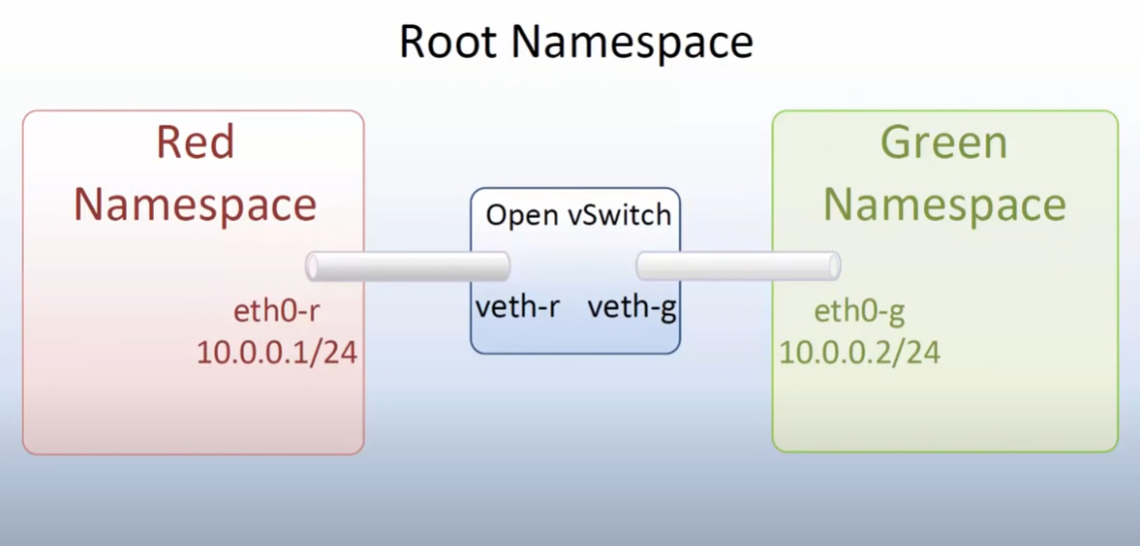
\includegraphics[width=14cm, keepaspectratio]{img/Linux namespaces}
		\caption{Resultado de crear un escenario con Linux Namespaces}
		\label{figura:linux_namespaces}
	\end{figure}
	
	Los comandos que se han utilizado para la definición de los espacios de nombres de red en Linux son:
	
	\begin{itemize}
		\item \verb*|ip link|: muestra una lista de todas las interfaces de red disponibles en el sistema, incluyendo tanto las disponibles como las no disponibles.
		
		\item \verb*|ip address|: muestra una lista de todas las direcciones IP asociadas con las interfaces de red de un sistema.
		
		\item \verb*|ip route|: muestra la tabla de enrutamiento del kernel, que determina cómo se dirigen los paquetes de red a través de la red.
		
		\item \verb*|ip netns add red|: crea un nuevo espacio de nombres de red llamado ''red'', donde posteriormente se podrán añadir interfaces de red, tablas de enrutamiento, etc. 
		
		\item \verb*|ip netns|: muestra el listado de espacios de nombres de red, para comprobar que se han creado correctamente.
		
		\item \verb*|ip netns exec red ip link|: Ejecuta el comando ip link dentro del espacio de nombres de red llamado ''red''. 
			
		\item \verb*|ovs-vsctl add-br OVS1|: Crea un nuevo Open vSwitch que se utiliza para conectar múltiples interfaces de red virtuales y permitir la comunicación entre ellas. 
				
		\item \verb*|ip link add eth0-r type veth peer name veth-r|:  crea un cable de red virtual tipo veth (Virtual Ethernet). Este cable virtual tiene dos extremos: eth0-r y veth-r.
		
		\item \verb*|ip link set eth0-r netns red|: conecta un extremo de red virtual (eth0-r) a un espacio de nombres de red específico (red). 
		
		\item \verb*|ovs-vsctl add-port OVS1 veth-r|: agrega el extremo del cable veth-r a OVS1. Como previamente se había conectado el extremo eth0-r al espacio de nombres de red "red", al ejecutar este comando dicho espacio de nombres quedará conectado a OVS1.
		
		\item \verb*|ip link set veth0-r up|: activa una interfaz de red virtual. En este caso, se activa la interfaz de red virtual llamada "veth0-r". Permitiendo que pueda transmitir y recibir datos. 
		
		\item \verb*|ip netns exec red ip link set dev eth0-r up|: activa la interfaz de red eth0-r dentro del namespace red.
		
		\item \verb*|ip netns exec red ip address add 10.0.0.1/24 dev eth0-r|: agrega una dirección IP a la interfaz de red eth0-r dentro del espacio de nombres de red llamado ''red''.
		
		
		
		
		
		
	
	\end{itemize}
	
	Utilizando estos comandos se crea un escenario simple con dos namespaces, ''red'' y ''green'', conectados a través de un switch virtual tal y como se muestra en la figura 3.1 Cada espacio de nombres tiene su tabla de encaminamiento independiente y diferente de la tabla de encaminamiento del espacio de nombres de red raíz que se corresponde con los recursos de la red de la máquina real.
	

	
	
	\section{Introducción a Mininet}
	
	Mininet permite la creación de espacios de nombres de red de forma más sencilla y su conexión a través
	de dispositivos Open vSwitch a través de un programa en Python. Mininet ofrece una interfaz sencilla
	de programación para la creación de máquinas (que se crean con espacios de nombres de red) y su
	configuración IP, así como la creación de enlaces entre las mismas.
	Una configuración similar a la representada en la figura 4.1 se obtiene en Mininet con el siguiente
	programa en Python:
	
	 \begin{lstlisting}[caption={Ejemplo de topología simple en Mininet}, label={lst:mytopo}]
	 	from mininet.topo import Topo
	 	
	 	class MyTopo( Topo ):
	 	"Simple topology example."
	 	
	 	def __init__( self ):
	 	"Create custom topo."
	 	# Initialize topology
	 	Topo.__init__( self )
	 	
	 	# Add hosts and switches
	 	redHost = self.addHost( 'red', ip='10.0.0.1/24' )
	 	greenHost = self.addHost( 'green', ip='10.0.0.2/24' )
	 	ovs1 = self.addSwitch( 'OVS1' )
	 	
	 	# Add links
	 	self.addLink( redHost, ovs1 )
	 	self.addLink( greenHost, ovs1 )
	 	
	 	topos = { 'mytopo': ( lambda: MyTopo() ) }
	 \end{lstlisting}
	
	La función addHost crea un espacio de nombres de red denominado "red" al que le configura
	la dirección IP 10.0.0.1/24. Esta misma función se utiliza para crear el espacio de nombres de
	red llamado "green" con la dirección IP 10.0.0.2/24.
	La función addSwitch crea un Open vSwitch llamado "OVS1". A continuación crea cables virtuales
	para conectar el Open vSwitch con los espacios de nombres "red" y "green" a través de la función
	addLink.
	
	AÑADIR POSIBLE IMAGEN DE MININET
	
	Como se ha podido demostrar, el uso de Mininet permite programar de forma sencilla
	topologías de red gracias a la interfaz de programación en Python. Configurar manualmente
	los espacios de nombres de red sería muy complicado cuando se desean escenarios con
	muchos dispositivos conectados entre ellos. Por este motivo, Mininet se usa como herramienta
	para la emulación de topologías de red en las que probar protocolos de comunicaciones.
	
	
	
	%%%%%%%%%%%%%%%%%%%%%%%%%%%%%%%%%%%%%%%%%%%%%%%%%%%%%%%%%%%%%%%%%%%%%%%%%%%%%%%%
	%%%%%%%%%%%%%%%%%%%%%%%%%%%%%%%%%%%%%%%%%%%%%%%%%%%%%%%%%%%%%%%%%%%%%%%%%%%%%%%%
	% ESTUDIO Y ANÁLISIS DEL PLANO DE CONTROL EN BANDA PERIPLUS %
	%%%%%%%%%%%%%%%%%%%%%%%%%%%%%%%%%%%%%%%%%%%%%%%%%%%%%%%%%%%%%%%%%%%%%%%%%%%%%%%%
	\cleardoublepage % empezamos en página impar
	\chapter{Estudio y análisis del plano de control Periplus} % título del capítulo (se muestra)
	\label{chap:periplus} % identificador del capítulo (no se muestra, es para poder referenciarlo)
	
	Este Trabajo de Fin de Grado se centra principalmente en el plano de control in-band que genera el controlador Periplus. Este plano de control está desarrollado en Python por el Grupo de Investigación de Alto Rendimiento en Tecnologías de la Información y Comunicaciones para el Desarrollo Humano de la Universidad Rey Juan Carlos. Periplus es un controlador in-band, es decir, que utiliza la misma infraestructura tanto para el plano de datos como para el plano de control. Partiendo de una configuración inicial mínima, los switches OpenFlow deben descubrir donde
	se encuentra el controlador para establecer una conexión TCP que permita definir la sesión
	OpenFlow. Una vez establecida esa sesión Periplus podrá instalar en los switches la configuración
	necesaria para el plano de control.
	
	Para ello, Periplus utiliza mecanismos como Proxy ARP y Anycast que facilitan el descubrimiento de la máquina en la que se encuentra el controlador.
	
	Periplus busca aumentar la robustez del plano de control permitiendo que los switches reaccionen rápidamente a fallos en enlaces y switches sin necesidad de esperar nuevas instrucciones del controlador, ya que los propios mensajes tienen información de las posibles rutas alternativas cuando falle un enlace.
	Además. se minimiza la cantidad de flujos almacenados en los switches que admiten el plano de control, ya que la información de enrutamiento no se almacena en los switches, sino en los caminos que van encapsulados en los paquetes intercambiados en el plano de control.
	
	
	\section{Inicialización de la Comunicación Controlador-Switch}
	
	El proceso de inicialización de la comunicación entre un controlador SDN y los switches es esencial para garantizar el funcionamiento coordinado de la red. Este proceso incluye varias etapas clave, cada una de las cuales es crucial para establecer una red operativa y gestionable. A continuación, se presenta una descripción detallada de este proceso:
	
	\subsection{Descubrimiento del Controlador}
	\begin{itemize}
		\item Los switches, al encenderse, deben establecer una conexión TCP con el controlador SDN. Esta conexión se utilizará para establecer la sesión OpenFlow entre cada switch y el controlador.
		\item Para enviar mensajes al controlador, el switch primero necesita conocer su dirección MAC. El primer mensaje que un switch enviará será una solicitud ARP para obtener la dirección Ethernet del nodo donde está el controlador.
	\end{itemize}
	Si el switch que está arrancando está directamente conectado al controlador o a otro
	switch que ya está gestionado por el controlador, el nuevo switch recibirá la respuesta
	de ARP que le permitirá conectarse 	con el controlador. Si no fuera así, el nuevo switch
	deberá esperar 	a que un  switch vecino	esté gestionado	por el	controlador.
	
	\subsection{Establecimiento de la Sesión OpenFlow}
	El controlador y cada uno de los switches establecen una sesión OpenFlow para intercambiar mensajes de configuración. Esto incluye la configuración inicial de los flujos OpenFlow que definen el comportamiento básico de los switches.

	
	\subsection{Intercambio inicial de características}
	\begin{itemize}
		\item \textbf{Reporte de características}: Los switches informan al controlador sobre sus características, como el número de puertos y características específicas del hardware.
		\item \textbf{Evaluación por el Controlador}: El controlador utiliza esta información para optimizar las decisiones de enrutamiento y gestión de flujos.
	\end{itemize}
	
	El controlador va obteniendo la información de la topología completa de la red y podrá calcular los caminos mas cortos entre cada switch y el controlador y viceversa, aplicando Dijkstra.
	
	\subsection{Instalación de Flujos para encaminamiento}
	\begin{itemize}
		\item \textbf{Definición de Flujos Básicos}: El controlador envía flujos iniciales a los switches, que permiten definir el comportamiento del switch cuando éste tiene que enviar un mensaje al contorlador o cuando el switch tiene que reenviar un mensaje a un determinado destino.
		\item \textbf{Implementación en los Switches}: Los switches aplican estas reglas en sus tablas de flujo, para implementar la función de encaminamiento.
	\end{itemize}
	
	\subsection{Monitorización de la red}
		El controlador monitorea la red y ajusta los flujos instalados en los switches si se producen cambios en la red.
	
	\section{Flujo OpenFlow}
	Vamos a describir el flujo normal de OpenFlow cuando se arranca un escenario desde cero. Este proceso implica la conexión inicial entre el controlador y el switch, así como la configuración de reglas de flujo. Aquí están los pasos típicos:
	
	\begin{itemize}
		\item Inicio del Controlador y Switches:
		\begin{itemize}
			\item El controlador SDN y los switches OpenFlow se inician.
			\item Los switches establecen conexiones TCP con el controlador.
		\end{itemize}
		
		\item Handshake Inicial:
		\begin{itemize}
			\item Los switches envían mensajes OFPT\_HELLO para iniciar el handshake con el controlador.
			\item El controlador responde con mensajes OFPT\_HELLO.
		\end{itemize}
		
		\item Negociación de Características (Feature Negotiation):
		\begin{itemize}
			\item Después del handshake, el controlador puede enviar mensajes OFPT\_FEATURES\_REQUEST
			a cada switch para obtener información sobre sus características y capacidades.
			\item Cada switch responde con mensajes OFPT\_FEATURES\_REPLY, proporcionando detalles como
			el número de puertos y las capacidades compatibles.
		\end{itemize}
		
		\item Configuración de Flujo Inicial:
		\begin{itemize}
			\item El controlador envía mensajes OFPT\_FLOW\_MOD a los switches para configurar reglas
			de flujo iniciales.
			\item Estas reglas especifican cómo se deben manejar ciertos tipos de tráfico en la red.
		\end{itemize}
		
		\item Establecimiento de Conexiones entre Switches:
		\begin{itemize}
			\item Si hay múltiples switches en la red, el controlador puede enviar mensajes
			OFPT\_FLOW\_MOD para configurar reglas de flujo que definen cómo los switches deben
			comunicarse entre sí.
		\end{itemize}
		
		\item Manejo de Paquetes:
		\begin{itemize}
			\item Cuando un switch recibe un paquete, verifica las reglas de flujo en su tabla de
			flujo para determinar cómo manejarlo.
			\item Si no hay reglas coincidentes, el switch puede enviar el paquete al controlador
			mediante un mensaje OFPT\_PACKET\_IN.
		\end{itemize}
		
		\item Pruebas de Conexión con ECHO:
		\begin{itemize}
			\item El controlador puede enviar mensajes OFPT\_ECHO\_REQUEST para realizar pruebas de conexión. Esto indica si ha habido alguna desconexión o problema de conexión en alguno de los switches si no hay respuesta en un tiempo relativamente corto.
			\item Cada switch responde a los mensajes OFPT\_ECHO\_REQUEST con mensajes OFPT\_ECHO\_REPLY.
		\end{itemize}
		
		\item Actualizaciones Dinámicas de Reglas:
		\begin{itemize}
			\item A medida que cambian las condiciones de la red o se producen eventos específicos,
			el controlador puede enviar mensajes OFPT\_FLOW\_MOD adicionales para actualizar
			dinámicamente las reglas de flujo en los switches.
		\end{itemize}
	\end{itemize}
	
	\section{Encaminamiento Basado en Origen}
	Periplus utiliza un modelo de encaminamiento basado en origen. Los nodos que se comunican insertan en los mensajes el camino que deben seguir para llegar al destino, y los nodos intermedios extraen esta información para reenviar los mensajes. El controlador ha calculado un camino principal y
	posibles caminos alternativos desde cada nodo al controlador y viceversa. Los flujos que instala el controlador en los switches
	permiten insertar estos	caminos	en los mensajes	que	envía cada switch.
	
	Para calcular los caminos, el controlador construye un árbol virtual con la raíz en el nodo origen. Este árbol permite calcular los caminos más cortos para la comunicación entre el controlador y los switches.

	
	PASAR ESTO A TABLA Para indicar el procso de como un nuevo switch quede gestionado por el controlador.
	\begin{itemize}
		\item \textbf{Envío de Solicitud ARP}: El switch nuevo envía solicitudes ARP por todos sus puertos. Si un switch vecino ya está gestionado, reenvía esta solicitud al controlador encapsulada en un mensaje OpenFlow.
		\item \textbf{Respuesta de ARP}: El controlador responde a la solicitud ARP a través del switch ancla, que la envía de vuelta al switch nuevo.
		\item \textbf{Establecimiento de la Conexión TCP}: Con la dirección MAC del controlador conocida, el switch nuevo establece una conexión TCP, permitiendo la sesión OpenFlow.
		\item \textbf{Configuración de Flujos}: El controlador instala los flujos necesarios en el switch nuevo para integrarlo completamente en la red gestionada.
	\end{itemize}
		
	La comunicación entre los nodos ya gestionados y el controlador se lleva a cabo mediante un proceso sofisticado de encaminamiento en origen, diseñado para establecer una comunicación tolerante a fallos en una red definida por software. 
	
	El controlador genera un "grafo" que representa la ruta completa que un paquete debe seguir para llegar desde un switch hasta el controlador, o viceversa, y el grafo se inserta en cada mensaje que un se intercambian los switches y el controlador. Así, cada paquete transporta consigo la información necesaria para su encaminamiento a lo largo de la red.
	
	El controlador configura los flujos OpenFlow en cada switch gestionado para que incluyan estos grafos en las una cabecera adicional de los paquetes. Esto implica definir reglas específicas en los switches para interpretar y procesar adecuadamente la información del Grafo contenida en las cabeceras adicionales de los paquetes. De esta manera, los switches intermedios interpretan la información de enrutamiento que se incluye en los mensajes.
	
	Para transmitir esta información de encaminamiento, se utiliza la cabecera NSH (Network Service Headers) que se situa entre las cabeceras de nivel 2 y 3. Aunque el protocolo NSH se utiliza típicamente para la comunicación entre controladores SDN, en este contexto se reutiliza de manera innovadora como un contenedor de información de encaminamiento. Esta adaptación permite transportar los grafos de encaminamiento a lo largo de la red.
	
	El grafo incluye un camino primario codificado como una lista de puertos de los switches en el camino, además de caminos alternativos utilizando la misma codificación.
	
	A continuación se muestra un ejemplo de condificación ded grafo.
	
	\begin{figure}[H]
		\centering
		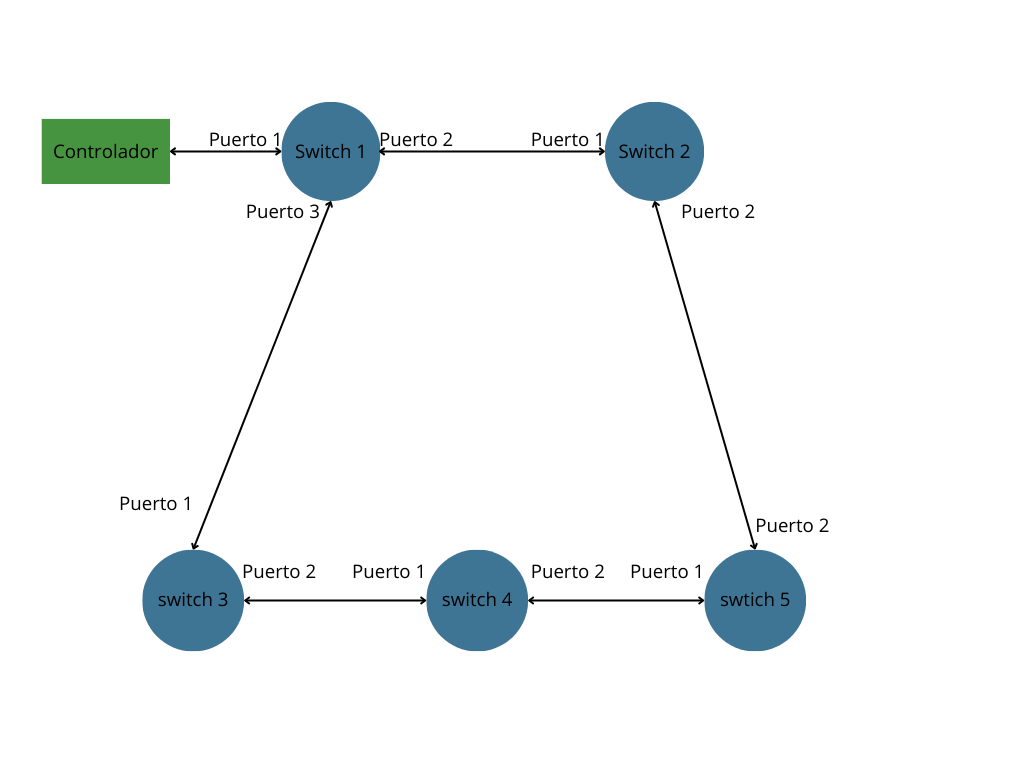
\includegraphics[width=16cm, keepaspectratio]{img/Ejemplo Periplus 1}
		\caption{Escenario formado por 5 switches y un nodo controlador}
		\label{figura:PeriplusEj1}
	\end{figure}
	
	Supongamos que tenemos un escenario simple con 5 switches y un controlador como el mostrado en la Figura 4.1. La comunicación entre el controlador y el switch 5 se puede realizar a través de 2 caminos posibles, uno más corto siguiendo la ruta controlador -> s1 -> s2 -> s5 y otro mas largo a través de controlador -> s1 -> s3 -> s4 -> s5. 
	
	El mensaje que sale de un nodo llevará en la cabecera NSH los números de puerto de salida de cada
	switch que indican el camino que debe llegar el mensaje desde el origen al destino.
	
	\begin{figure}[H]
		\centering
		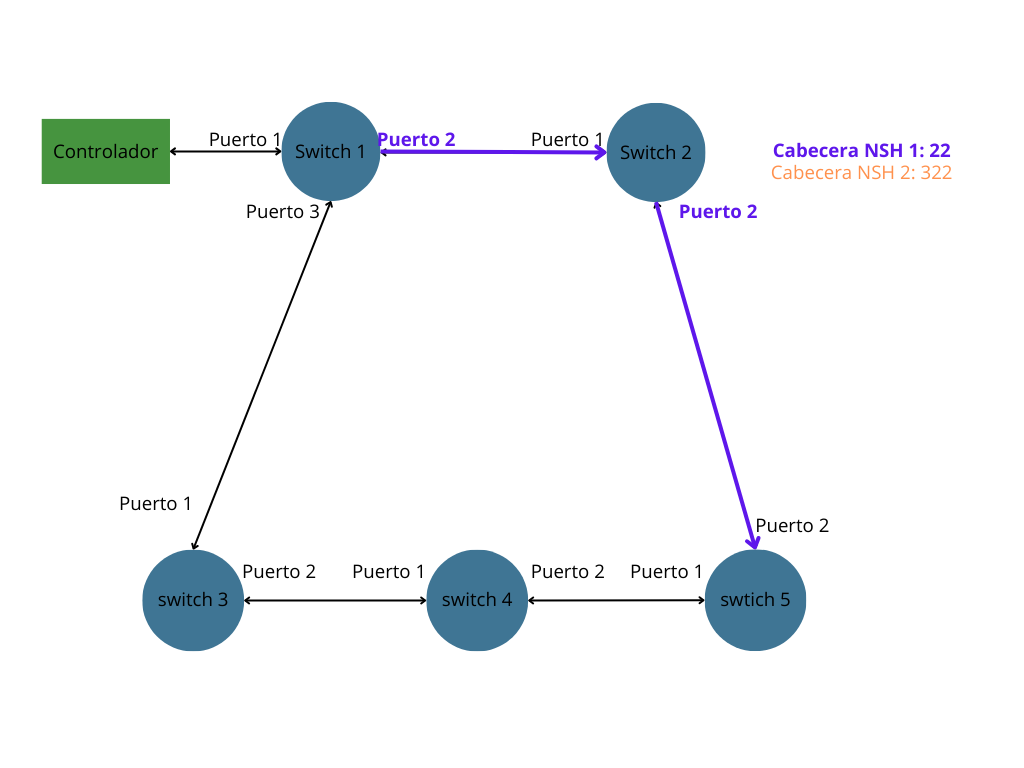
\includegraphics[width=16cm, keepaspectratio]{img/Ejemplo Periplus 2}
		\caption{Comunicación desde el controlador al switch 5.}
		\label{figura:PeriplusEj2}
	\end{figure}
	
	En el ejemplo que se muestra en la figura 5.2, el controlador desea enviar un mensaje
	al switch 5. El mensaje que enviará el controlador y que podrá capturarse en el enlace que une el
	controlador con el switch 1 debe llevar en la cabecera NSH el grafo que contiene
	los puertos de salida en cada switch para llegar al switch 5. En este caso,
	el grafo debe ser 22. Cuando el mensaje llegue al switch 1, éste debe eliminar del
	grafo el puerto por donde lo envía (puerto 2) y
	enviarlo a través de dicho puerto (puerto 2). Cuando le mensaje alcance el
	switch 2, éste debe eliminar del grafo el puerto por donde lo envía (puerto 2) y enviarlo
	a través de dicho puerto (puerto 2)- De esta forma el mensaje llegará a
	su destino.
	Adicionalmente, el mensaje que envíe el controlador contendrá también un camino alternativo
	por si se produce algún fallo en el camino principal. El camino alternativo en este caso queda
	definido por el grafo 322. Es decir, desde el switch 1 se envía a través del puerto 3, al llegar al
	switch 3 se envía a través del puerto 2 y al llegar al switch 4 se envía a través del puerto 2.


 \textcolor{blue}{Explica aquí que la codificación de los puertos se realiza en 4 bits y que el bit más significativo indica
que ese salto tiene un camino alternativo y que el útimo salto antepone 0xf.	
Para este caso la codificación del camino principal sería: 0xafa, siendo el primer salto el switch 1
desde el cuál el camino alternativo sería 0x32f2 y el segundo salto sería el switch s2 con camino alternativo
0x132f2}
	\begin{figure}[H]
		\centering
		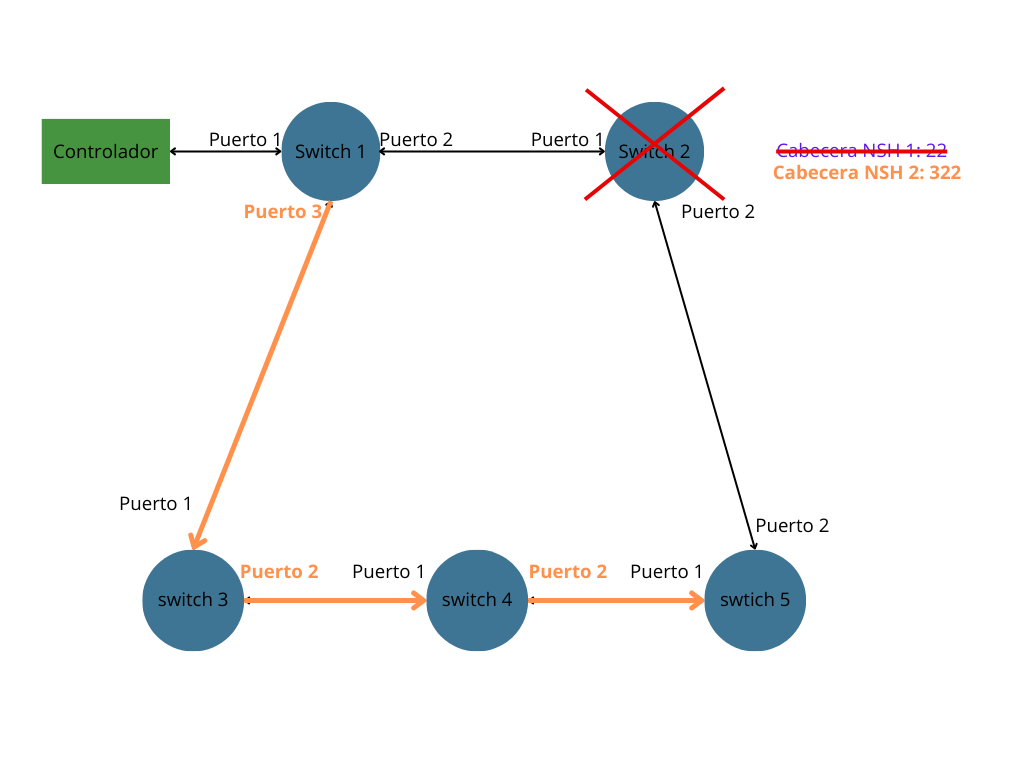
\includegraphics[width=16cm, keepaspectratio]{img/Ejemplo Periplus 3}
		\caption{Escenario de Ejemplo 3}
		\label{figura:PeriplusEj3}
	\end{figure}
	
	En el caso de que el Switch 2 o su enlace con el estuviera caido o no diera señales de estar activo, el switch 1 elegiría el camino alternativo, como se muestra en la Figura 5-3 marcado en color naranja.
	
	 \textcolor{blue}{Sería bueno que pudiéramos poner una imagen de wireshark con la cabecera NSH.}

	\section{Gestión de los switches: Tablas OpenFlow}
	
	En el proceso de gestión de los switches por parte del controlador en una red definida por software, se configuran las tablas OpenFlow en cada switch para garantizar un enrutamiento eficiente del tráfico de red. Estas tablas, divididas en varios niveles, determinan el flujo de los paquetes a través de la red.
	
	La primera tabla, denominada Tabla 0, es la primera en ser consultada por los paquetes entrantes. Su función principal es verificar si hay más saltos en el camino principal del paquete y, en caso afirmativo, almacenar la información del próximo salto en un registro específico. Luego, el paquete se reenvía a las Tablas 1 y 2 para un procesamiento adicional.
	
	La Tabla 1 se utilizaba en una implementación alternativa del controlador para la detección de puertos inactivos, pero en la implementación actual está vacía. Por otro lado, la Tabla 2 asigna el paquete a una "tabla de grupo". Esta tabla de grupo se encarga de detectar la actividad de los puertos mediante mensajes del protocolo Bidirectional Forwarding Detection(BFD) y, en función de ello, enviar el paquete a la Tabla 11 si el camino está activo, o continuar con el procesamiento en la Tabla 3.
	
	La Tabla 11, utilizada desde la tabla de grupo, almacena el puerto de salida activo en un registro y envía el paquete a la Tabla 3. Aquí, se desencapsula la cabecera NSH de los paquetes y se elimina el puerto actual de salida del grafo. Si el puerto está activo, el paquete se envía por ese puerto; de lo contrario, se consulta si existe un camino alternativo.
	
	Las Tablas 4 y 5 se utilizan en caso de que exista camino alternativo. Se elimina el camino principal de la cabecera NSH para sustituirlo por el camino alternativo almacenado en la siguiente cabecera NSH. A continuación, el paquete se reenvía a la Tabla 0 para su procesamiento posterior.
	
	En resumen, las tablas OpenFlow en los switches son configuradas y adaptadas por el controlador para facilitar un enrutamiento eficiente y flexible del tráfico de red, garantizando una comunicación fluida y adaptativa en entornos SDN.
	
	 \textcolor{blue}{Hacer diagrama de flujo que muestre el camino entre las diferentes tablas}
	
	%%%%%%%%%%%%%%%%%%%%%%%%%%%%%%%%%%%%%%%%%%%%%%%%%%%%%%%%%%%%%%%%%%%%%%%%%%%%%%%%
	%%%%%%%%%%%%%%%%%%%%%%%%%%%%%%%%%%%%%%%%%%%%%%%%%%%%%%%%%%%%%%%%%%%%%%%%%%%%%%%%
	% EXPERIMENTOS Y VALIDACIÓN %
	%%%%%%%%%%%%%%%%%%%%%%%%%%%%%%%%%%%%%%%%%%%%%%%%%%%%%%%%%%%%%%%%%%%%%%%%%%%%%%%%
	
	\cleardoublepage
	\chapter{Experimentos de arranque de Periplus en diferentes escenarios}
	\label{chap:experimentos}
	
 	A lo largo de este capítulo se va a realizarexperimentos de arranque de Periplus en 4 escenarios de red en los que configuraremos el uso de 1 controlador o varios controladores. Posteriormente se compararán los resultados en cuanto al tiempo de conexión de los switches con el o los controladores, analizando así cómo afecta a un escenario el añadir nuevos controladores.%
	 
	En este capítulo, se realizarán diversos cálculos y recogida de datos respecto a los tiempos de conexión de un conjunto de switches a sus controladores: 
	
	
	\begin{itemize}
		\item Se recogerá el tiempo que tardan en conectarse todos los switches. Con esta información podemos saber el tiempo que tarda el escenario en estar operativo. Muy útil principalmente para comparar tiempos entre escenarios con uno y varios controladores.
		
		\item Se recogerá la información de qué switches tiene conectado cada controlador. Muy descriptivo para ver cómo funcionan los escenarios con multicontrolador. Esto nos indicará el reparto de switches por controlador, observando además que, como era de esperar, a mayor cercanía del controlador, más posibilidades de estar conectado a dicho controlador.
		
		\item El camino que ha seguido cada switch para conectarse a su controlador. Con este estudio podemos ver en qué orden se han ido conectando los switches.
		
	\end{itemize}
 	
 	\clearpage
 	\section{Escenario 1}
 	En la figura 5.1 se muestra la conexión de un controlador
	ejecutándose en una máquina que tiene configurada la dirección
 	IP 10.0.0.1 y 8 switches. Junto a la interfaz Ethernet de cada switch
 	se muestra el número de puerto al que se corresponde dicha interfaz.
 	Los switches tienen configuradas las siguientes direcciones IP:
 	
 	\vspace*{-18pt}
 	%Figura Escenario 1 con 1 controlador
 	\begin{figure}[H]
 		\centering
 		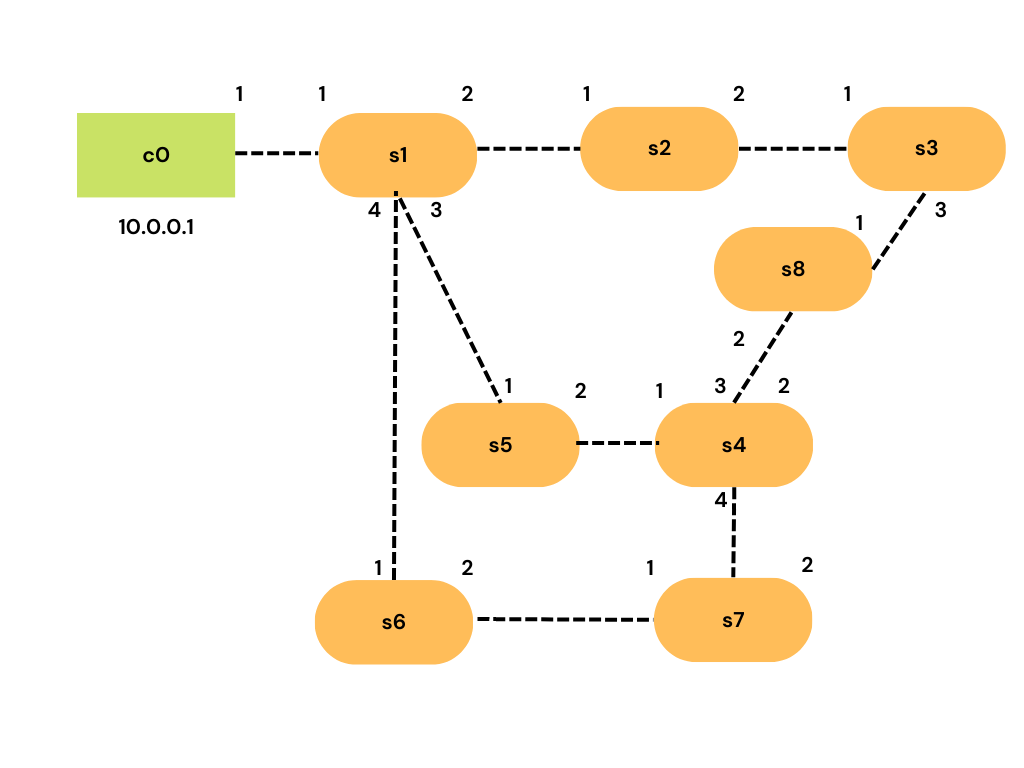
\includegraphics[width=12cm, keepaspectratio]{img/escenario1-1}
 		\caption{Escenario con un controlador y 8 switches}
 		\label{figura:escenario1-1c}
 	\end{figure}
 	
 	%Figura Escenario 1 con 1 controlador explicado
 	\begin{figure}[H]
 		\centering
 		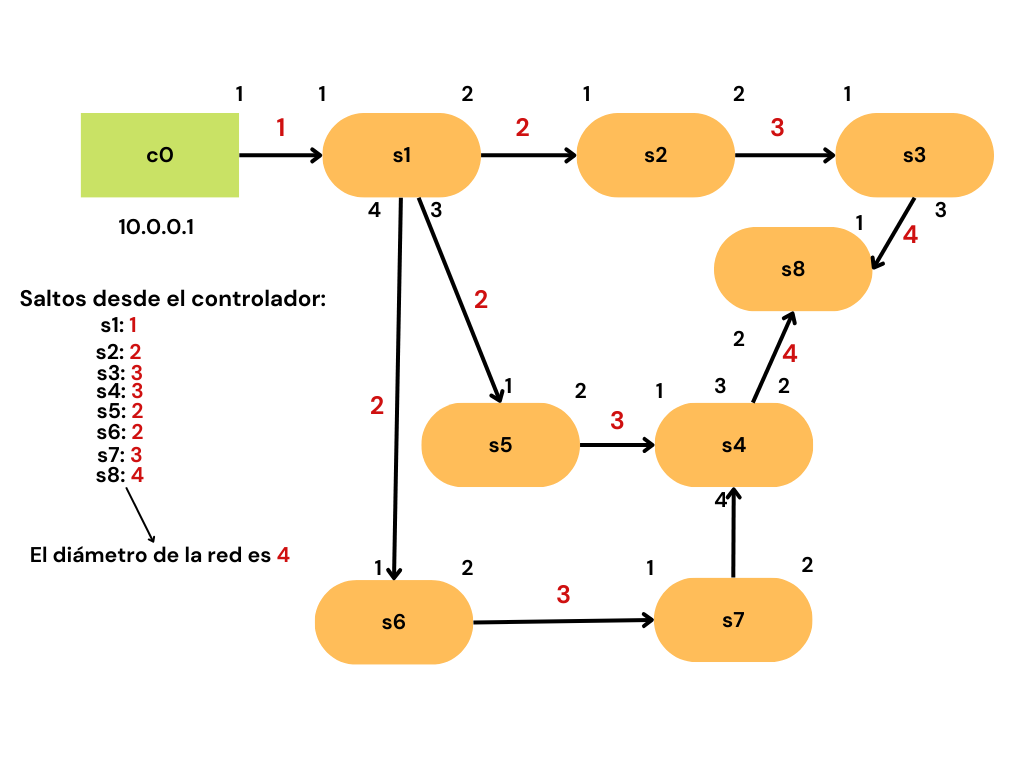
\includegraphics[width=12cm, keepaspectratio]{img/escenario1-explicado}
 		\caption{Primer escenario con 1 controlador explicado}
 		\label{figura:escenario1-explicado}
 		\vspace{-18pt}
 	\end{figure}
 	
 	En la figura 5.3 se muestra la misma topología de la figura 5.1 pero con 2 controladores: c0 y c1.
 	
 	%Figura Escenario 1 con 2 controladores
 	\begin{figure}[H]
 		\centering
 		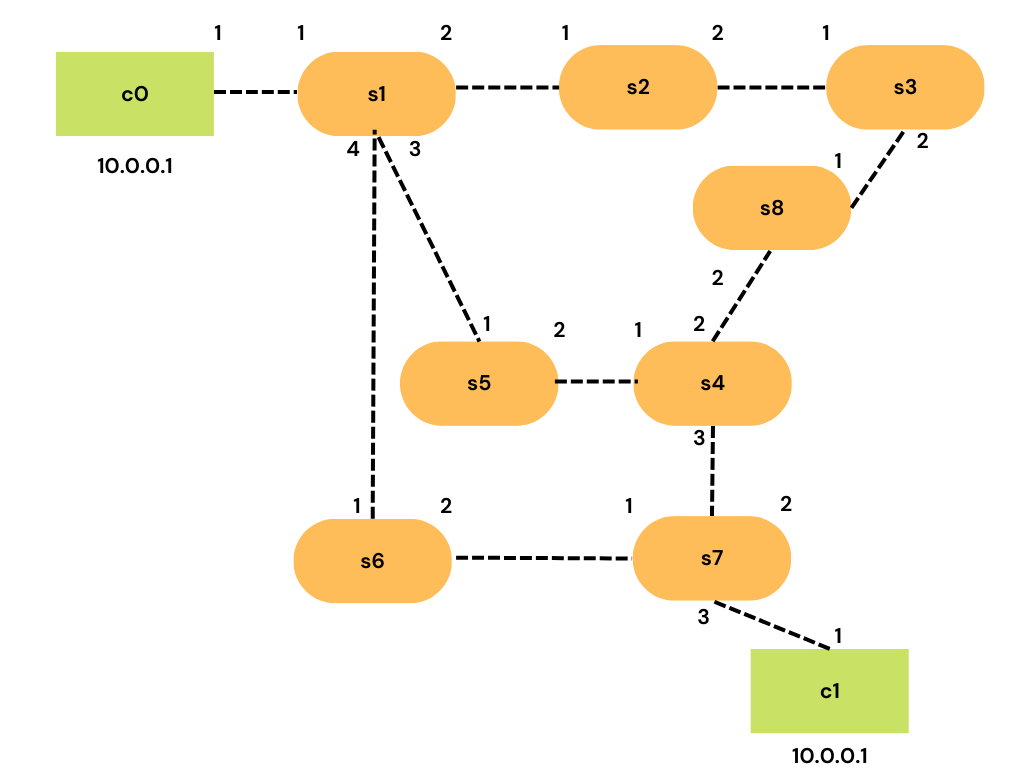
\includegraphics[width=12cm, keepaspectratio]{img/escenario1-2}
 		\caption{Primer escenario con 2 controladores}
 		\label{figura:escenario1-2c}
 		\vspace{-18pt}
 	\end{figure}
 	
 	 Al añadir un segundo controlador en el otro extremo del escenario, los switches deberían conectarse al controlador más cercano en número de saltos. Por tanto, los switches	 s1, s2, s3 y s5 deberían conectarse al controlador c0 y los switches s7, s4 y s8 al controlador c1. El switch
 	 s6 está a igual distancia de ambos controladores, por lo que podría conectarse tanto a c0 como a c1.
 	 
 	 A continuación se han realizado medidas para ver el tiempo que tardan los switches en estar gestionados por un controlador tanto en el escenario con 1 controlador, como en el de 2 controladores.
 	
 En la figura 5.4 se muestran los resultados obtenidos. La agregación de nuevos controladores a un escenario reducirá los tiempos máximos de conexión. La media de mejora en este escenario es de 0.0546 segundos, siendo esto una mejora del 14.59 \% al añadir un controlador extra al escenario. 
 	Estos resultados coinciden con lo que se esperaba previamente, ya que hay una mejoría, pero no es demasiado grande con respecto al mismo escenario con un solo controlador.
 	
 	%Figura comparativa de tiempos en el primer escenario
 	\begin{figure}[H]
 		\centering
 		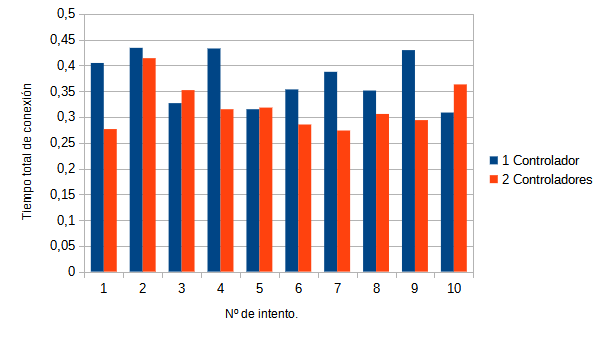
\includegraphics[width=16cm, keepaspectratio]{img/comparativabucle4}
 		\caption{Tiempo que tardan todos los switches del escenario 1 en estar gestionados por un controlador.}
 		\label{figura:comparativabucle4}
 	\end{figure}
 	
 	%Figura comparativa de medias en el primer escenario
 	\begin{figure}[H]
 		\centering
 		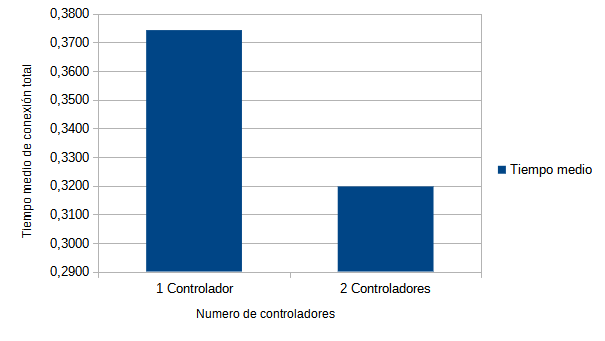
\includegraphics[width=12cm, keepaspectratio]{img/comparativamediasbucle}
 		\caption{Comparativa de media de tiempos en conseguir que todos los switches del escenario 1 estén gestionados por un controlador}
 		\label{figura:mediabucle4}
 	\end{figure}
 	
 	
 	Y como vemos en las siguientes gráficas, también hay bastante diferencia en la mediana y la varianza. Ya que al haber 2 controladores, es difícil que haya tiempos muy altos, de ahí que se reduzca la mediana y la varianza.
 	
 	
 	\begin{figure}[H]
 		\centering
 		
 		\subfigure[Comparativa de medianas en conseguir que todos los switches del escenario 1 estén gestionados por un controlador]{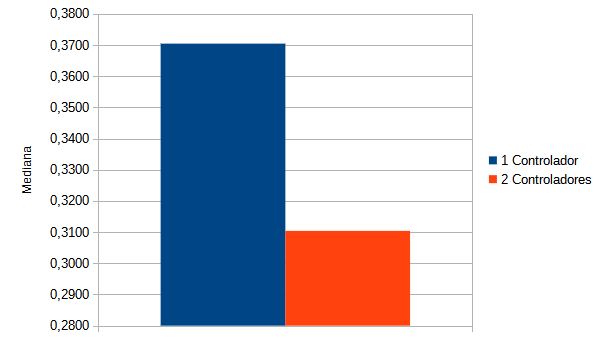
\includegraphics[width=0.45\textwidth]{img/comparativamedianabucle}}
 		\hfill
 		\subfigure[Comparativa de varianza en conseguir que todos los switches estén gestionados por un controlador]{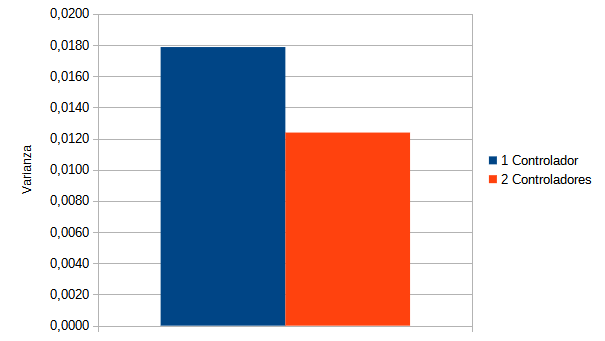
\includegraphics[width=0.45\textwidth]{img/comparativavarianzabucle}}
 		\hfill
 	\end{figure}
 	
 	Con el objetivo de ilustrar como cambia el escenario al añadir un controlador extra, se van a comparar los dos experimentos, viendo como se han ido conectando los switches paso a paso.
 	
 	Para el caso de 1 controlador, los esquemas se han ido conectando de las siguientes formas:
 	
 	\begin{figure}[H]
 		\centering
 		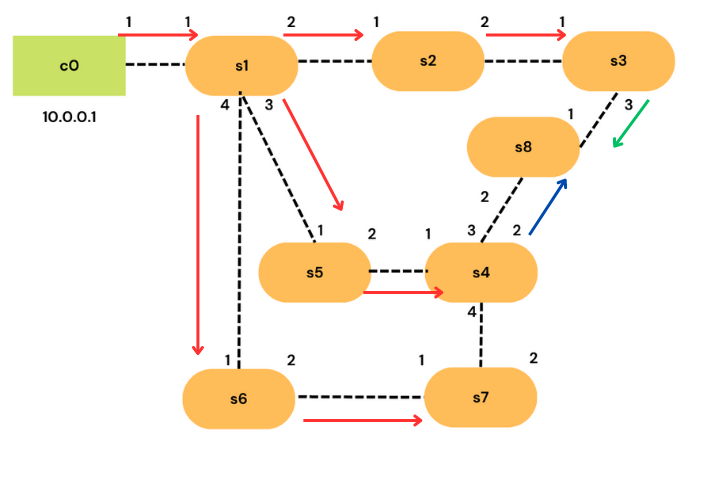
\includegraphics[width=12cm, keepaspectratio]{img/rutasEscenario1-1c}
 		\caption{Orden de conexión de los switches. El color rojo indica las conexiones que siempre se han realizado en las 10 ejecuciones}
 		\label{figura:escenario1_1c_1}
 	\end{figure}
 	
 	Las diferencias entre las ejecuciones se encuentran en el switch s8 que puede alcanzar
 	el controlador con el mismo coste en número de saltos a través de 2 caminos diferentes.
 	En las pruebas realizadas, en 2 ejecuciones s8 se conectó a través de s3 (camino verde
 	en la figura 5.6)	y en 8 ejecuciones s8 se conectó a través de s4 (camino	azul).
 	
 	Para el caso de 2 controladores, los resultados son muy variados, como se muestra en la siguiente figura:
 	
 	\begin{figure}[H]
 		\centering
 		
 		\subfigure[Orden de conexión de los experimentos 1, 4]{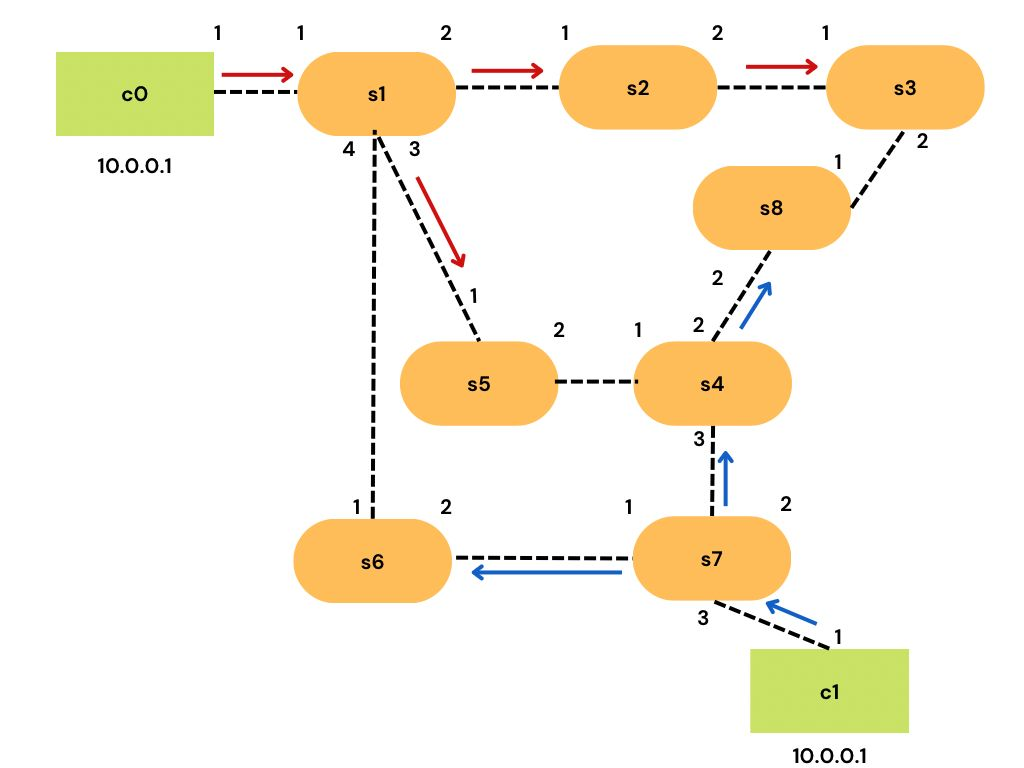
\includegraphics[width=0.45\textwidth]{img/escenario1_2c_1}}
 		\hfill
 		\subfigure[Orden de conexión de los experimentos 2, 9]{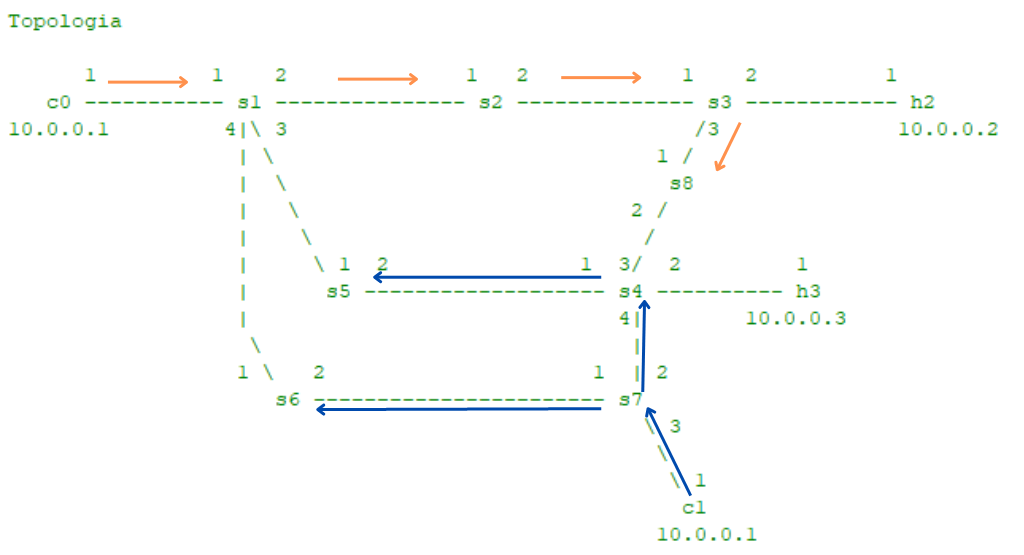
\includegraphics[width=0.45\textwidth]{img/escenario1_2c_2}}
 		\hfill
 		\vspace{10pt} % Ajusta el espacio vertical entre las filas
 		\subfigure[Orden de conexión del experimento 3]{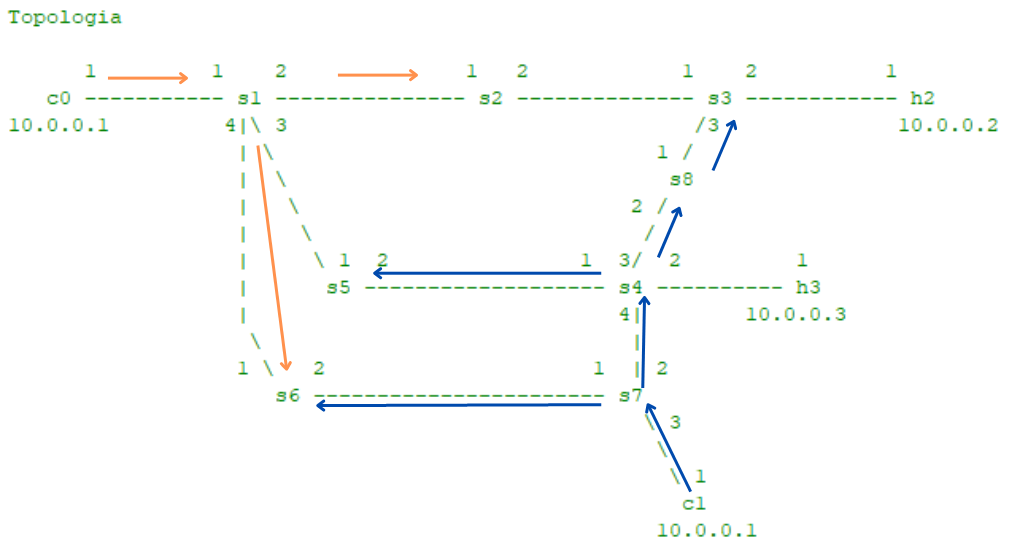
\includegraphics[width=0.45\textwidth]{img/escenario1_2c_3}}
 		\subfigure[Orden de conexión del experimento 5]{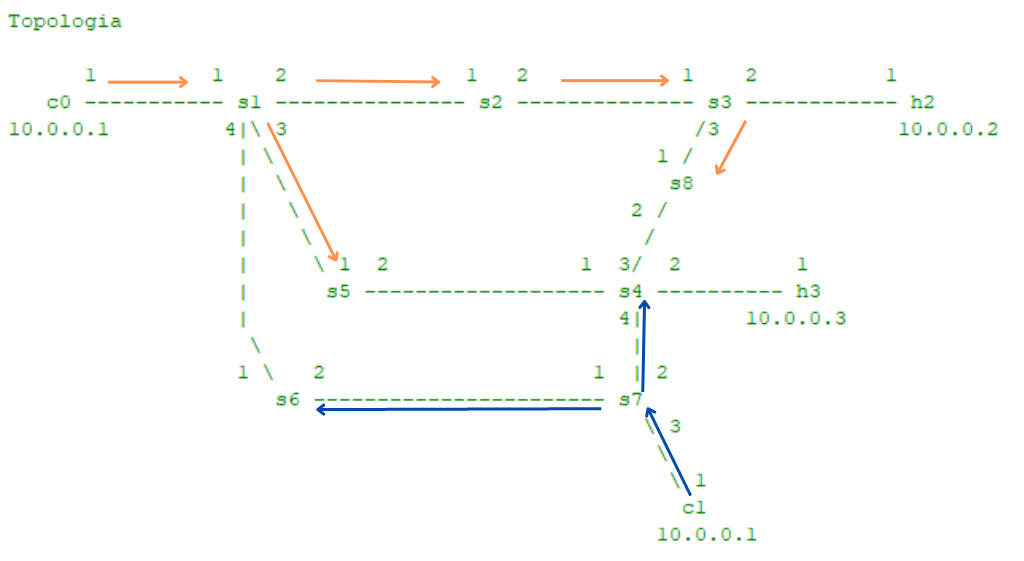
\includegraphics[width=0.45\textwidth]{img/escenario1_2c_4}}
 		\hfill
 		\vspace{10pt} % Ajusta el espacio vertical entre las filas
 		
 	
 		\subfigure[Orden de conexión del experimento 6]{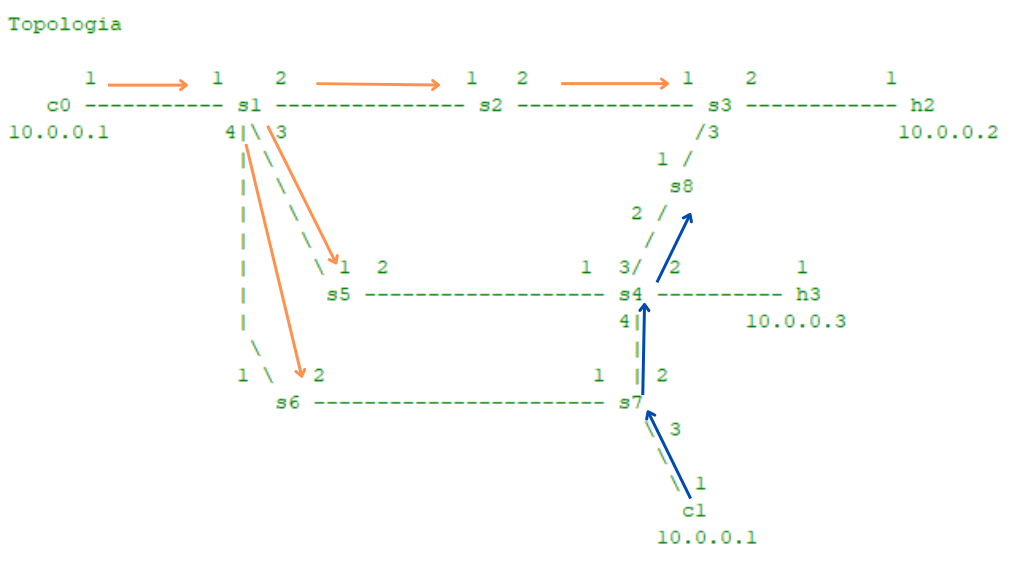
\includegraphics[width=0.45\textwidth]{img/escenario1_2c_5}}
 		\hfill
 		\subfigure[Orden de conexión del experimento 7]{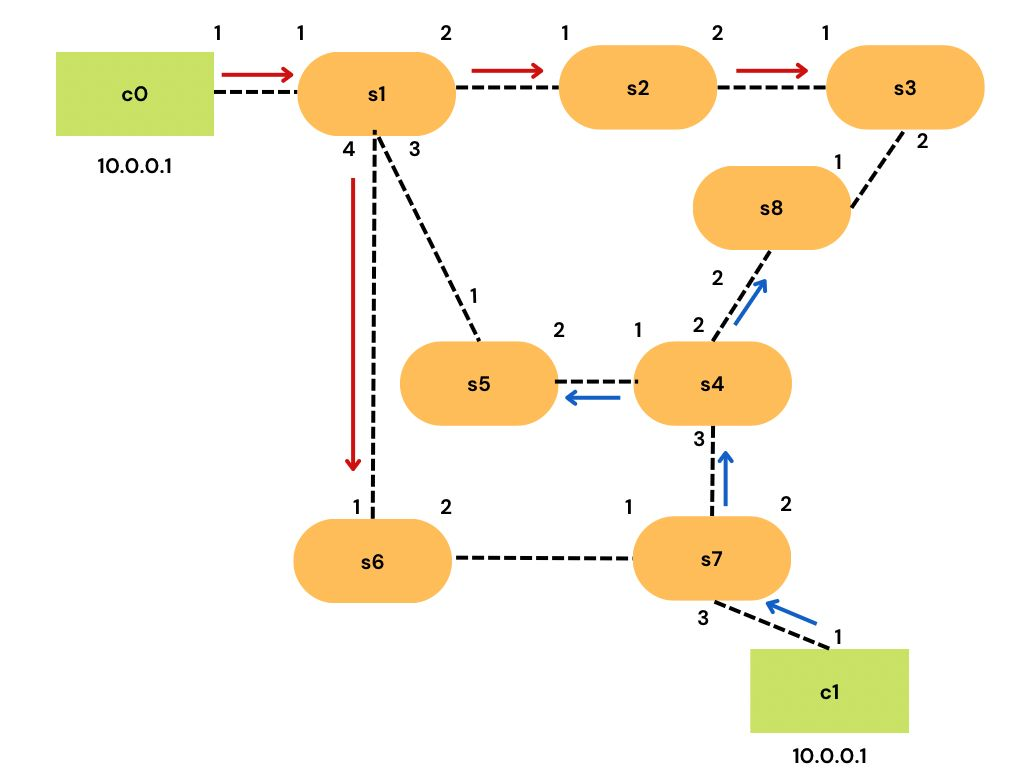
\includegraphics[width=0.45\textwidth]{img/escenario1_2c_6}}
 		
 		\vspace{10pt} % Ajusta el espacio vertical entre las filas
 		\subfigure[Orden de conexión del experimento 8]{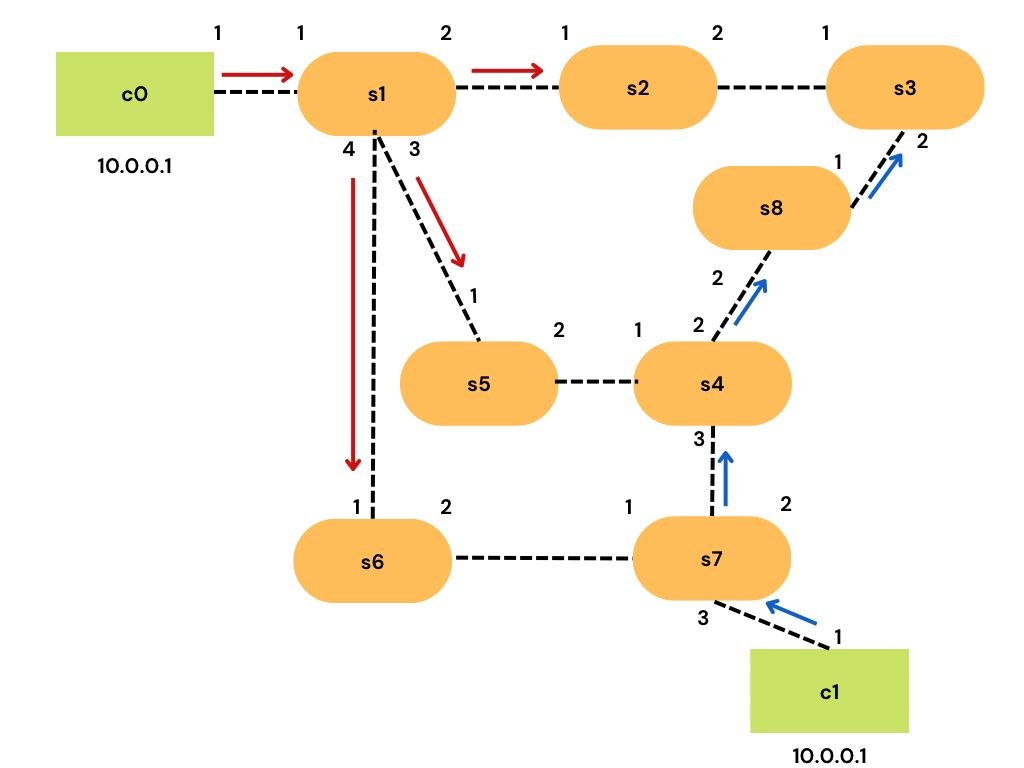
\includegraphics[width=0.45\textwidth]{img/escenario1_2c_7}}
 		\hfill
 		\subfigure[Orden de conexión del experimento 10]{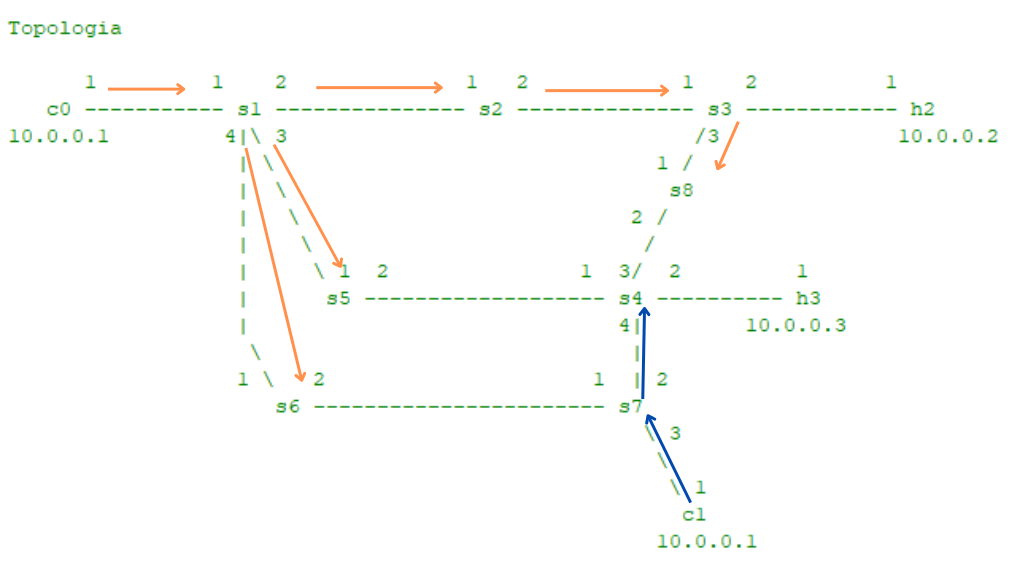
\includegraphics[width=0.45\textwidth]{img/escenario1_2c_8}}
 		
 		\caption{Conjunto de 8 imágenes}
 	\end{figure}
 	
 	Como podemos comprobar, pese a haber 10 experimentos, hemos podido ver 8 formas diferentes de conectar los switches. Algo que muestra la flexibilidad que tiene Periplus a la hora de realizar conexiones que en escenarios más grandes dará lugar a repartos equilibrados entre los controladores.
 	
 	El reparto de switches por controlador es homogéneo en la mayor parte de las 10 ejecuciones. En la última ejecución, como se puede ver en la figura 5.8 el reparto se ha realizado de forma muy diferente: 6 switches se han conectado al controlador c0 y 2 switches al controlador c1. Esto se debe a que el controlador c1 ha arrancado después con un pequeño retraso, dando el tiempo suficiente a que el controlador c0 haya ido avanzando con la asignación de switches. 
 	
 	\begin{figure}[H]
 		\centering
 		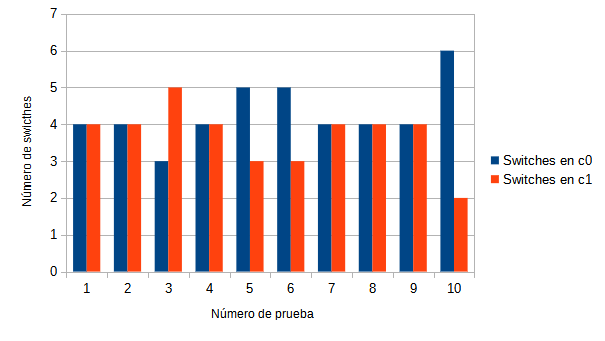
\includegraphics[width=16cm, keepaspectratio]{img/switchesporcontrollerescenario1}
 		\caption{Número de switches por controlador.}
 		\label{figura:switchesporcontrollerescenario1}
 	\end{figure}
 	
 	
 	
 	\clearpage
 	\section{Escenario 2}
 	
 	En la figura 5.9 se muestra un escenario más complejo formado por 16 switches y un único
 	controlador c0. La figura 5.10 muestra la misma topología con 4 controladores.
 		
 	En este escenario se espera una mejora muy superior en el tiempo de conexión de todos los switches a un controlador, ya que en el ejemplo con 1 controlador hay hasta 6 saltos hasta el switch mas lejano, y con 4 controladores se reduce a 3, por lo que a priori podríamos esperar una mejora bastante superior a la obtenida en el primer escenario.
 	
 	\begin{figure}[H]
 		\centering
 		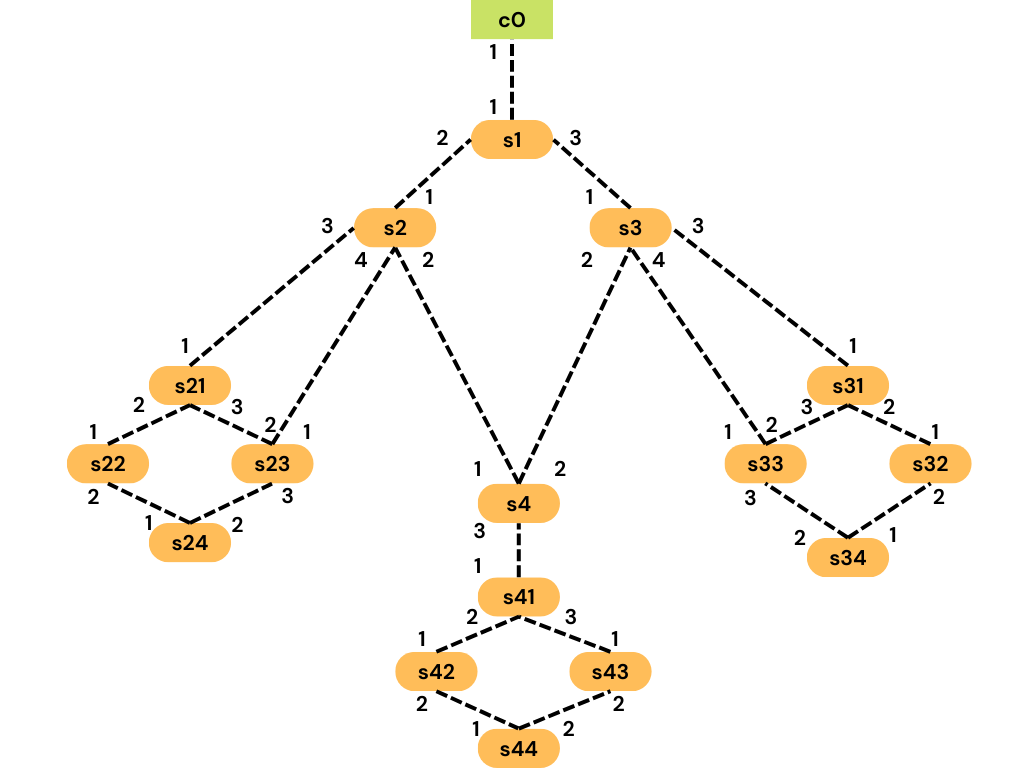
\includegraphics[width=14cm, keepaspectratio]{img/escenario2-1}
 		\caption{Segundo escenario con 1 controlador y 16 switches}
 		\label{figura:escenario2-1c}
 	\end{figure}
 	
 	\begin{figure}[H]
 		\centering
 		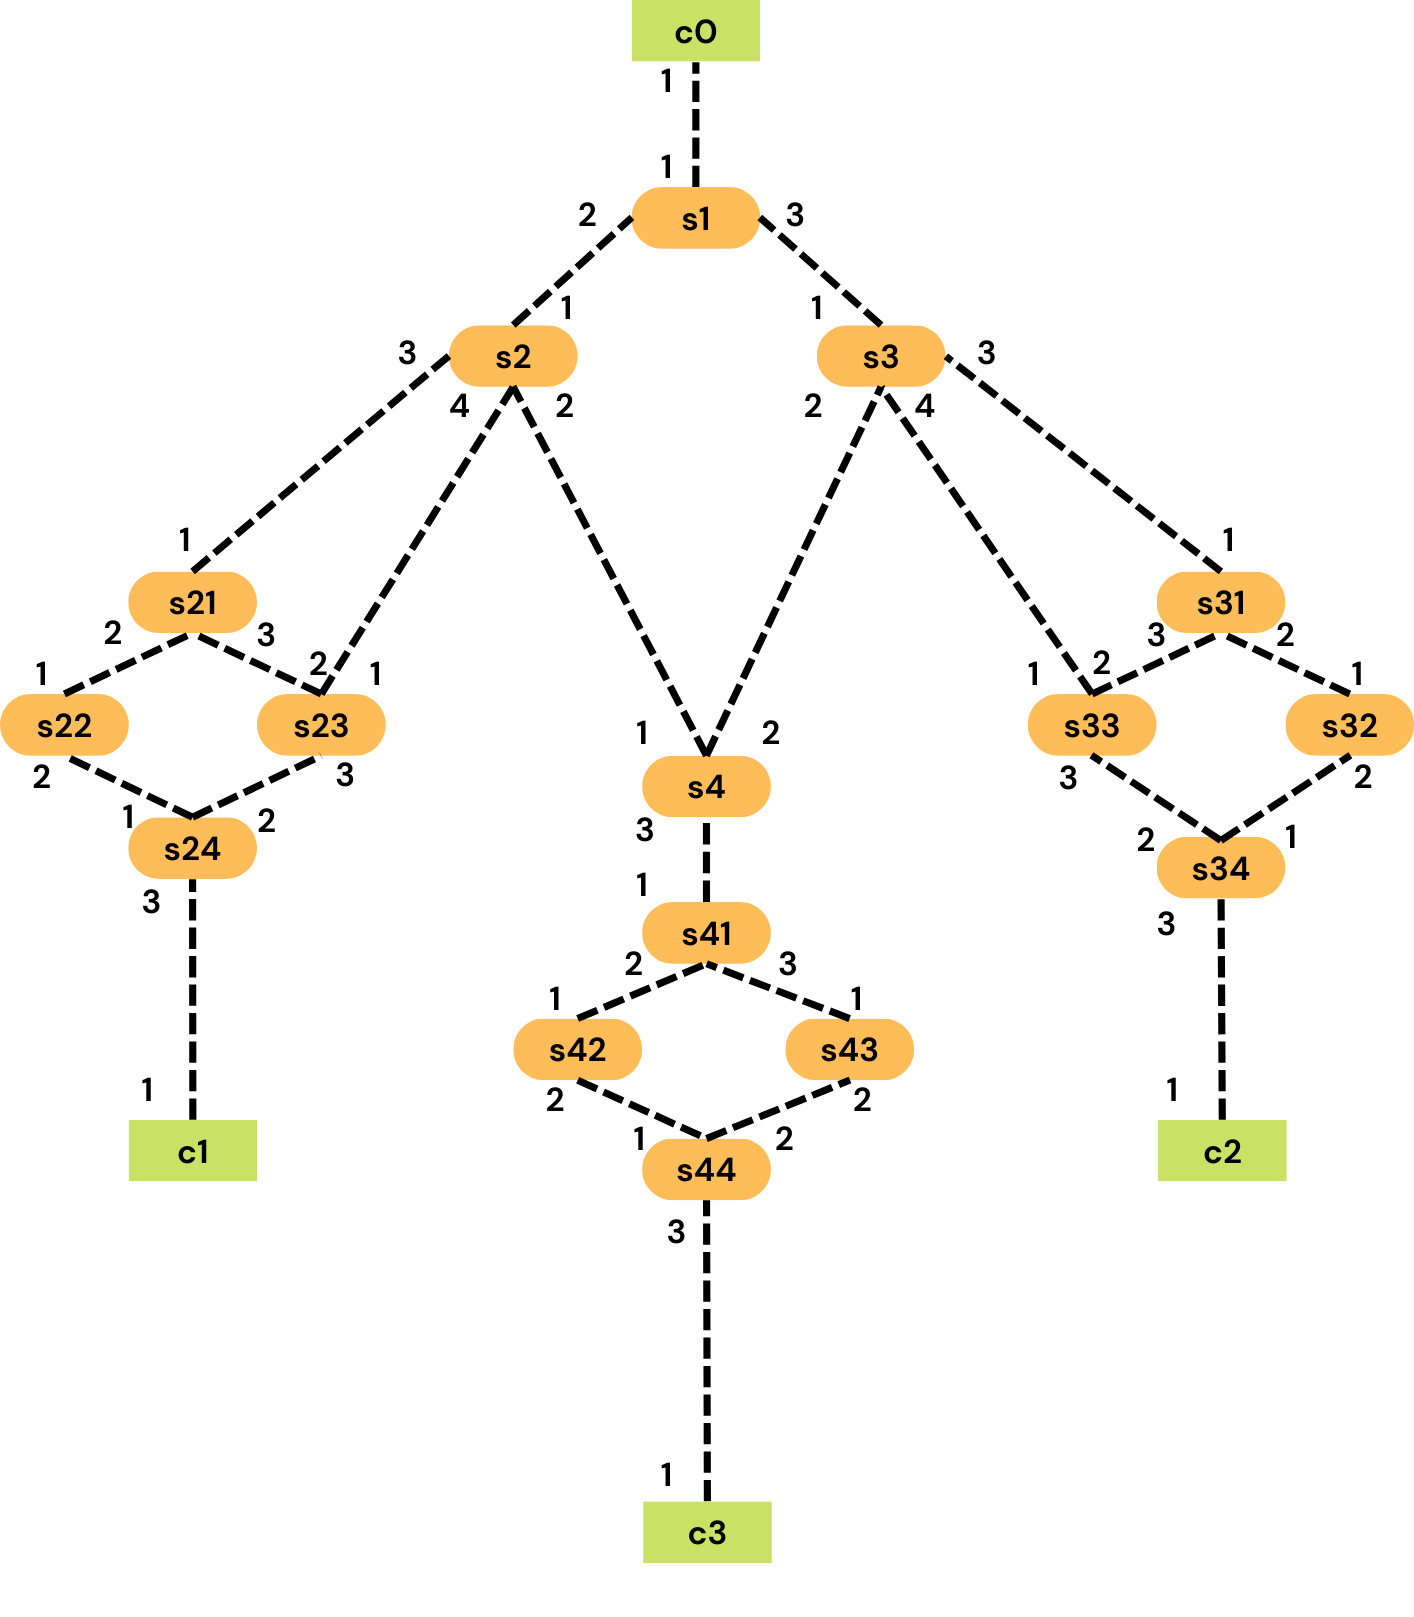
\includegraphics[width=14cm, keepaspectratio]{img/escenario2-2}
 		\caption{Segundo escenario con 4 controladores y 16 switches}
 		\label{figura:escenario2-4c}
 	\end{figure}
 	
 	Con estos resultados (figura 5.11, figura 5.12), podemos confirmar lo visto en el escenario 1 y lo que esperábamos antes de ver los resultados, ya que además en este escenario, al ser más grande y complejo, la disminución es mas notoria, ya que el tiempo máximo de conexión en los switches se ha reducido en 0.1464 segundos, siendo el sistema un 26.28 \% mas rápido con 4 controladores que con 1.
 	
 	%Figura comparativa de tiempos en el segundo escenario
 	\begin{figure}[H]
 		\centering
 		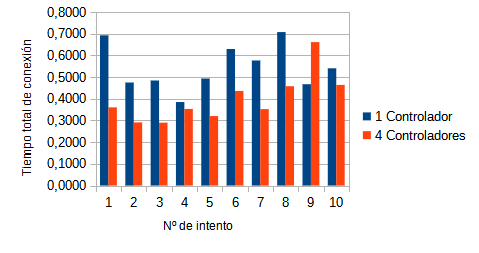
\includegraphics[width=16cm, keepaspectratio]{img/comparativamesh}
 		\caption{Tiempo que tardan todos los switches del escenario 2 en estar gestionados por un controlador.}
 		\label{figura:comparativamesh}
 	\end{figure}
 	
 	
 	%Figura comparativa de medias en el segundo escenario
 	\begin{figure}[H]
 		\centering
 		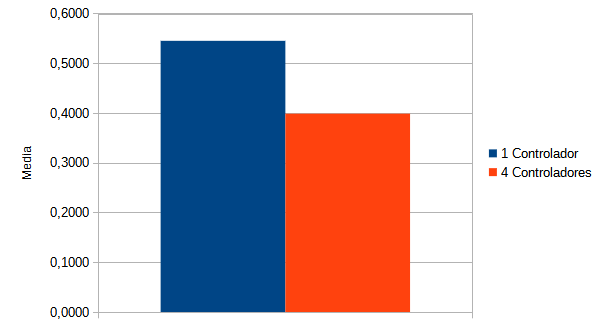
\includegraphics[width=12cm, keepaspectratio]{img/comparativamediamesh}
 		\caption{Comparativa de media de tiempos en conseguir que todos los switches del escenario 2 estén gestionados por un controlador.}
 		\label{figura:mediamesh}
 	\end{figure}
 	
 	
 	Y como puede verse en las siguientes gráficas, también hay bastante diferencia en la mediana y la varianza. Ya que al haber 4 controladores, es difícil que haya tiempos muy altos, de ahí que se reduzca la mediana y la varianza.
 	
 	\begin{figure}[H]
 		\centering
 		
 		\subfigure[Comparativa de medianas en conseguir que todos los switches del escenario 2 estén gestionados por un controlador]{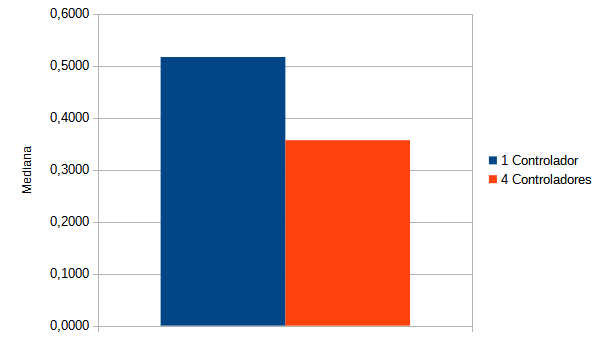
\includegraphics[width=0.45\textwidth]{img/comparativamedianamesh}}
 		\hfill
 		\subfigure[Comparativa de varianza en conseguir que todos los switches del escenario 2 estén gestionados por un controlador]{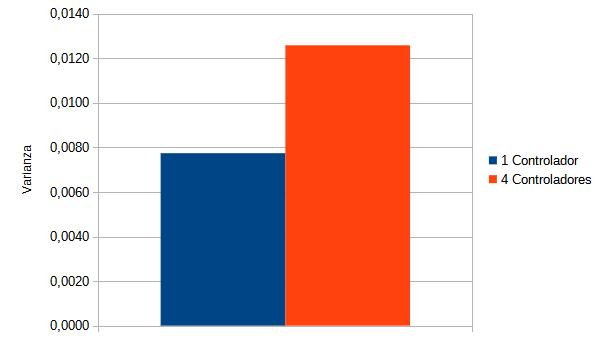
\includegraphics[width=0.45\textwidth]{img/comparativavarianzamesh}}
 		\hfill
 	\end{figure}
 	
 	
 	\vspace{10pt} 
 	
 	Además, hemos comprobado que por lo general el reparto de switches entre los controladores se ha realizado de forma bastante equitativa como puede verse en la figura 5.13. El reparto de los últimos experimentos se asocia a fallo de la máquina al realizar los experimentos, algo que ha ocurrido en los escenarios más grandes debido a la gran carga de trabajo que tenía el ordenador al realizar las simulaciones. 
 	
 	
 	\begin{figure}[H]
 		\centering
 		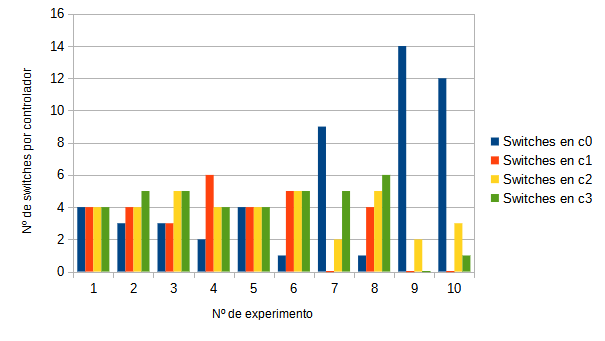
\includegraphics[width=16cm, keepaspectratio]{img/switchesporcontrollermesh}
 		\caption{Número de switches por controlador.}
 		\label{figura:switchesporcontrollermesh}
 	\end{figure}
 	
 	
 	\clearpage
 	\section{Escenario 3}
 	 
 	A continuación, se llevará a cabo un análisis de un escenario con caminos más complejos y largos (figura 5.14) y el mismo escenario con 2 controladores en vez de 1 (figura 5.15), para ver cómo reacciona Periplus en este caso.
 	En el escenario con un controlador, vemos que el switch mas lejano está a 4 saltos, mientras que el escenario con dos controladores el switch mas lejano está a 3 saltos. Lo curioso de este escenario es la gran cantidad de conexiones entre switches que hay, y que el segundo controlador se coloca en el extremo mas lejano, pero lejos de otra gran parte de los switches.
 	
 	%Figura comparativa de tiempos en el tercer escenario
 	\begin{figure}[H]
 		\centering
 		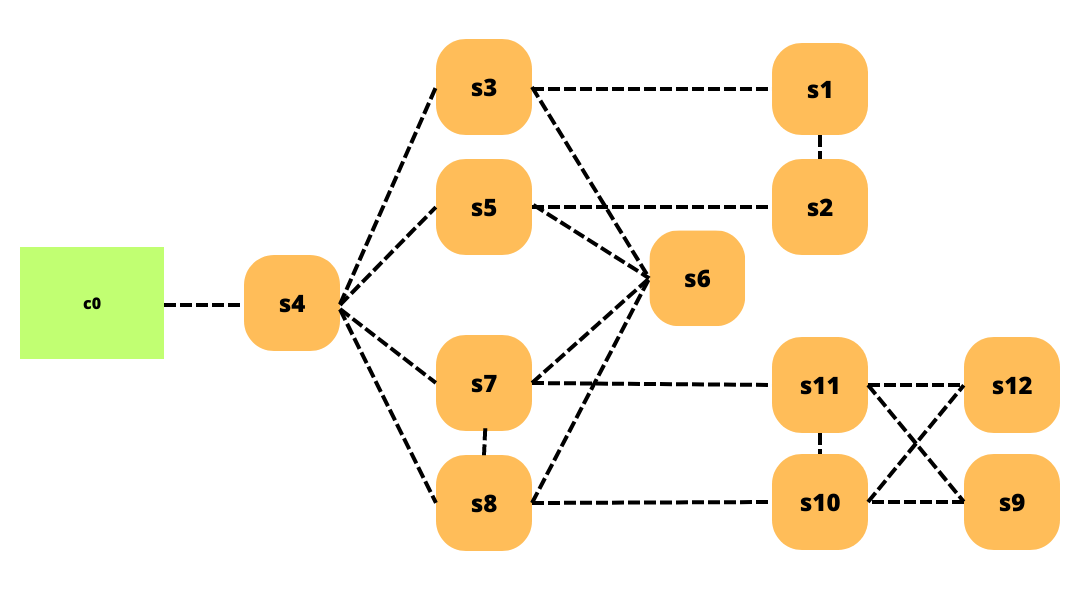
\includegraphics[width=14cm, keepaspectratio]{img/b4_1}
 		\caption{Tercer escenario con 1 controlador y 12 switches}
 		\label{figura:b4_1}
 	\end{figure}
 	
 	%Figura comparativa de medias en el tercer escenario
 	\begin{figure}[H]
 		\centering
 		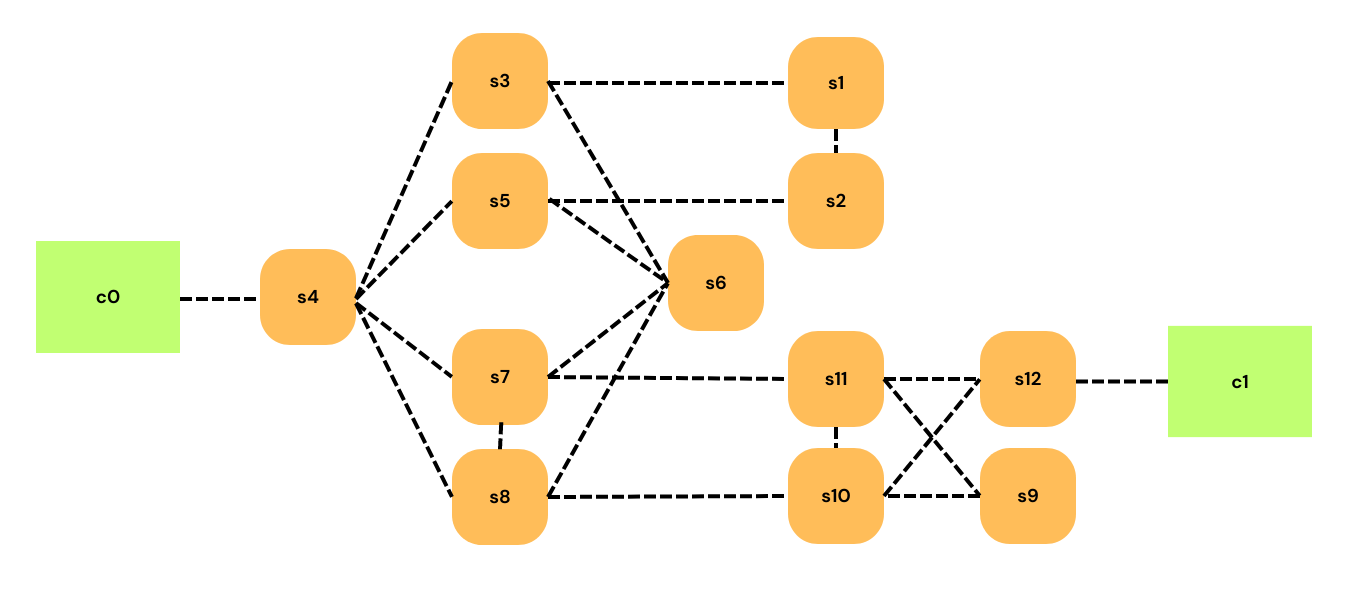
\includegraphics[width=14cm, keepaspectratio]{img/b4_2}
 		\caption{Tercer escenario con 2 controladores y 12 switches}
 		\label{figura:b4_2}
 	\end{figure}
 	
 	Con estos resultados(figura 5.16, figura 5.17), podemos confirmar lo visto en los anterior escenarios, ya que además en este escenario, al ser mas grande y complejo, la disminución es mas notoria, ya que el tiempo máximo de conexión en los switches se ha reducido en 0.168 segundos, siendo el sistema un 47.19 \% mas rápido con 2 controladores que con 1.
 	
 	Además comparando tiempos, se empieza a ver una tendencia, que cuantos mas saltos entre switches se reduzcan, mas efectivo es el circuito.
 	
 	\begin{figure}[H]
 		\centering
 		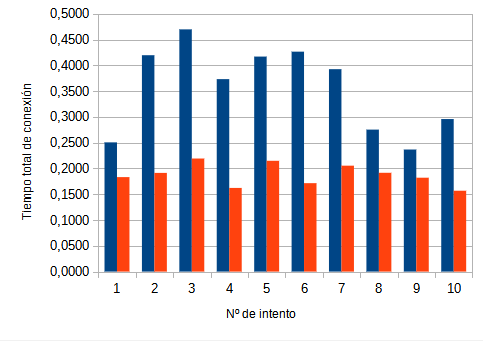
\includegraphics[width=12cm, keepaspectratio]{img/comparativaescenario3}
 		\caption{Comparativa de tiempos en el tercer escenario}
 		\label{figura:comparativab4}
 	\end{figure}
 	
 	
 	
 	\begin{figure}[H]
 		\centering
 		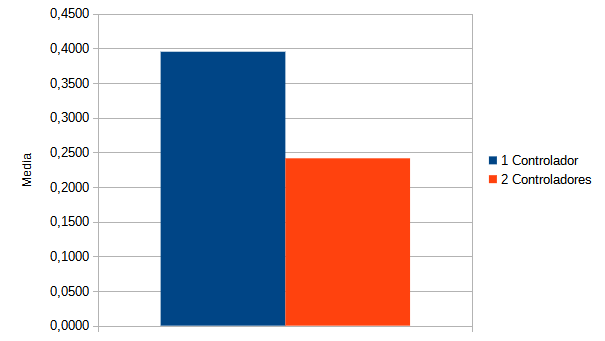
\includegraphics[width=12cm, keepaspectratio]{img/comparativamediaescenario3}
 		\caption{Comparativa de media de tiempos en el tercer escenario}
 		\label{figura:mediab4}
 	\end{figure}
 	
 	Y como vemos en las siguientes gráficas, también hay bastante diferencia en la mediana y la varianza. Ya que al haber 2 controladores y tanta conexión, es difícil que haya tiempos muy altos, de ahí que se reduzca la mediana y sobretodo la varianza.
 	
 	\begin{figure}[H]
 		\centering
 		
 		\subfigure[Comparativa de medianas en conseguir que todos los switches del escenario 3 estén gestionados por un controlador]{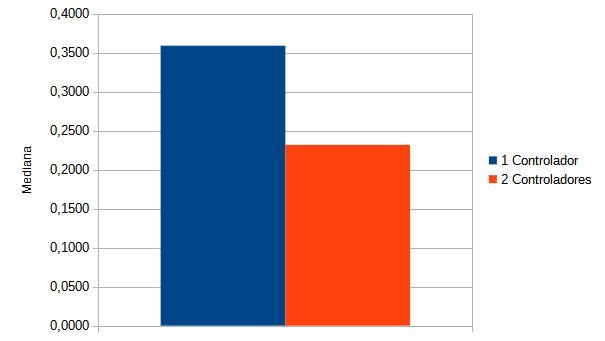
\includegraphics[width=0.45\textwidth]{img/comparativamedianaescenario3}}
 		\hfill
 		\subfigure[Comparativa de varianza en conseguir que todos los switches del escenario 3 estén gestionados por un controlador]{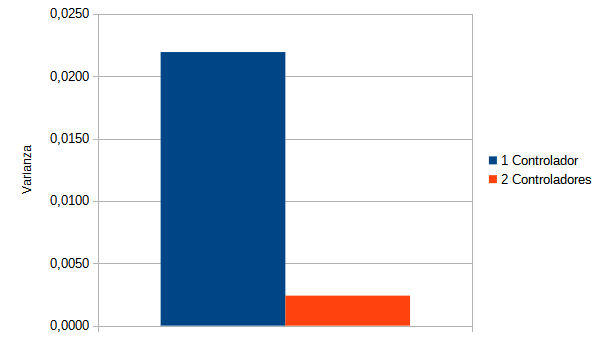
\includegraphics[width=0.45\textwidth]{img/comparativavarianzaescenario3}}
 		\hfill
 	\end{figure}
 	
 	
 	\clearpage
 	Además, viendo la figura 5.18 hemos comprobado que el reparto de switches entre los controladores se ha realizado de forma previsible y como se intuía al principio- El primer controlador acapara mas switches conectados en cada experimento, debido a que tiene una mayor cantidad de switches mas cerca que el segundo controlador.
 	
 	
 	\begin{figure}[H]
 		\centering
 		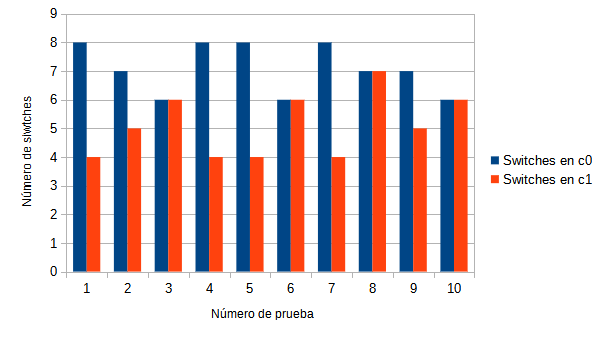
\includegraphics[width=16cm, keepaspectratio]{img/switchesporcontrollerescenario3}
 		\caption{Número de switches por controlador.}
 		\label{figura:switchesporcontrollerb4}
 	\end{figure}
	
	\clearpage
	\section{Escenario 4}
	
	En este último experimento y a diferencia de los escenarios anteriores, se realizará una tercera comparación, ya que estudiaremos un escenario con uno, dos, y cuatro controladores, para comprobar cómo cambia en función de cada caso.
	En la figura 5.19 podemos observar el primer caso, un unico controlador para 20 switches, en la figura 5.20 tenemos el mismo escenario pero con 2 controladores para los 20 switches y la figura 5.21 que es ésta vez tiene 4 controladores para los 20 switches.
	
	En este escenario, el numero de saltos no va a disminuir, ya que se va a mantener la misma distancia máxima entre los controladores y los switches mas alejados, pero se esperan tiempos mas bajos debido a que el reparto de trabajo se va a dividir por 2 y 4 respectivamente.
	
	\begin{figure}[H]
		\centering
		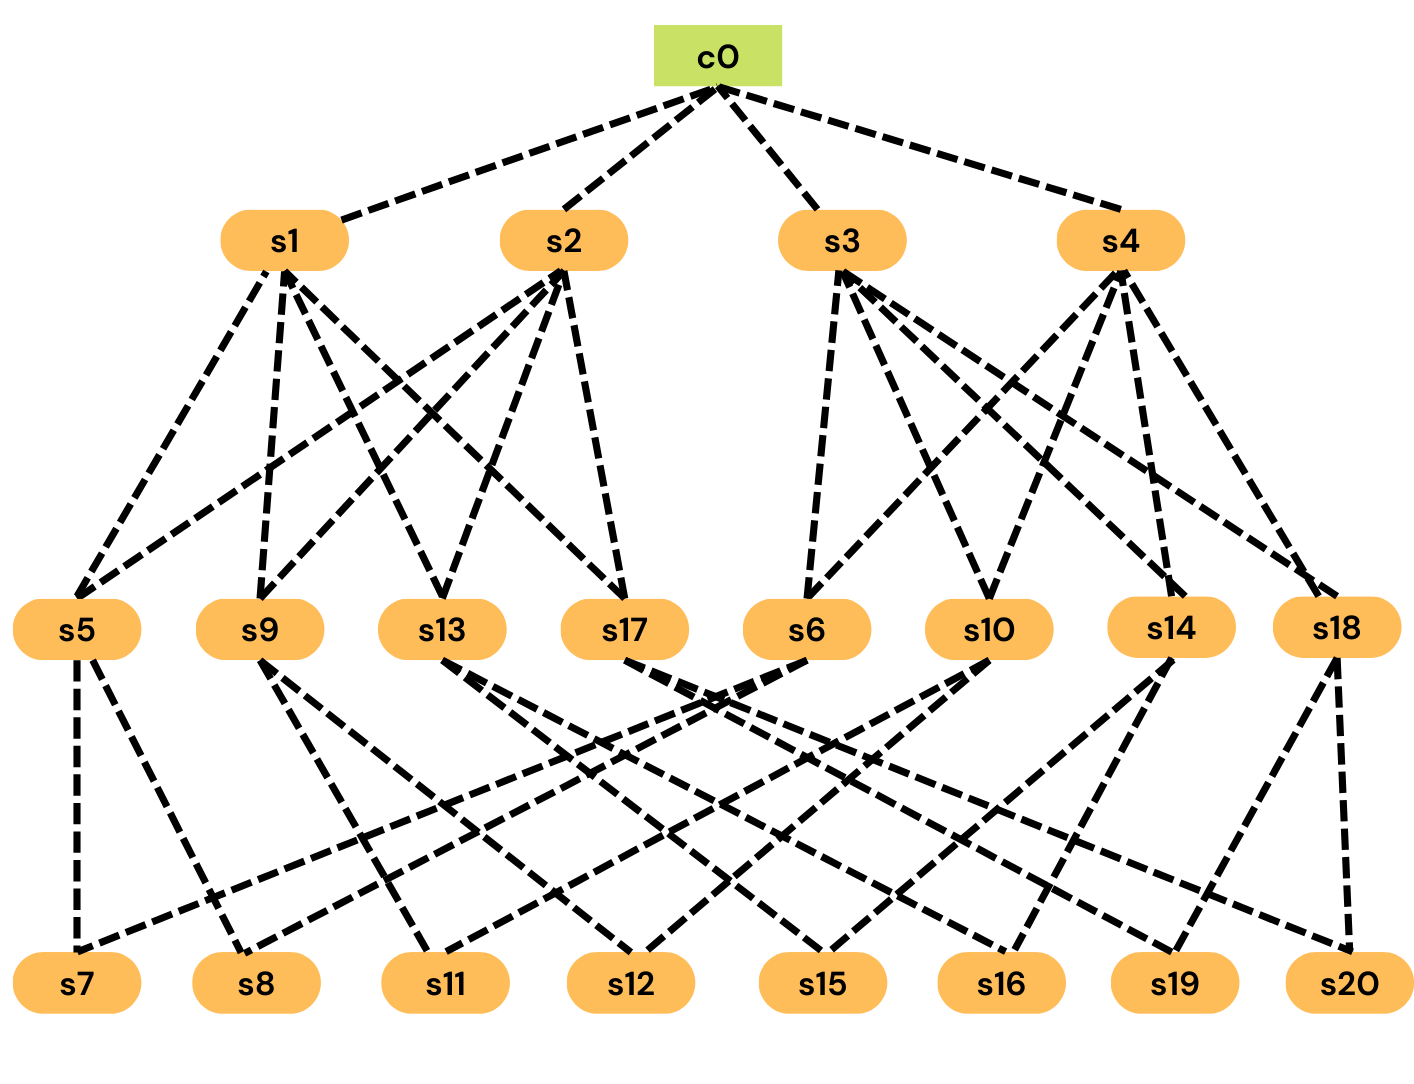
\includegraphics[width=16cm, keepaspectratio]{img/e4_1}
		\caption{Cuarto escenario con 1 controlador y 20 switches}
		\label{figura:e4_1}
	\end{figure}
	
	\begin{figure}[H]
		\centering
		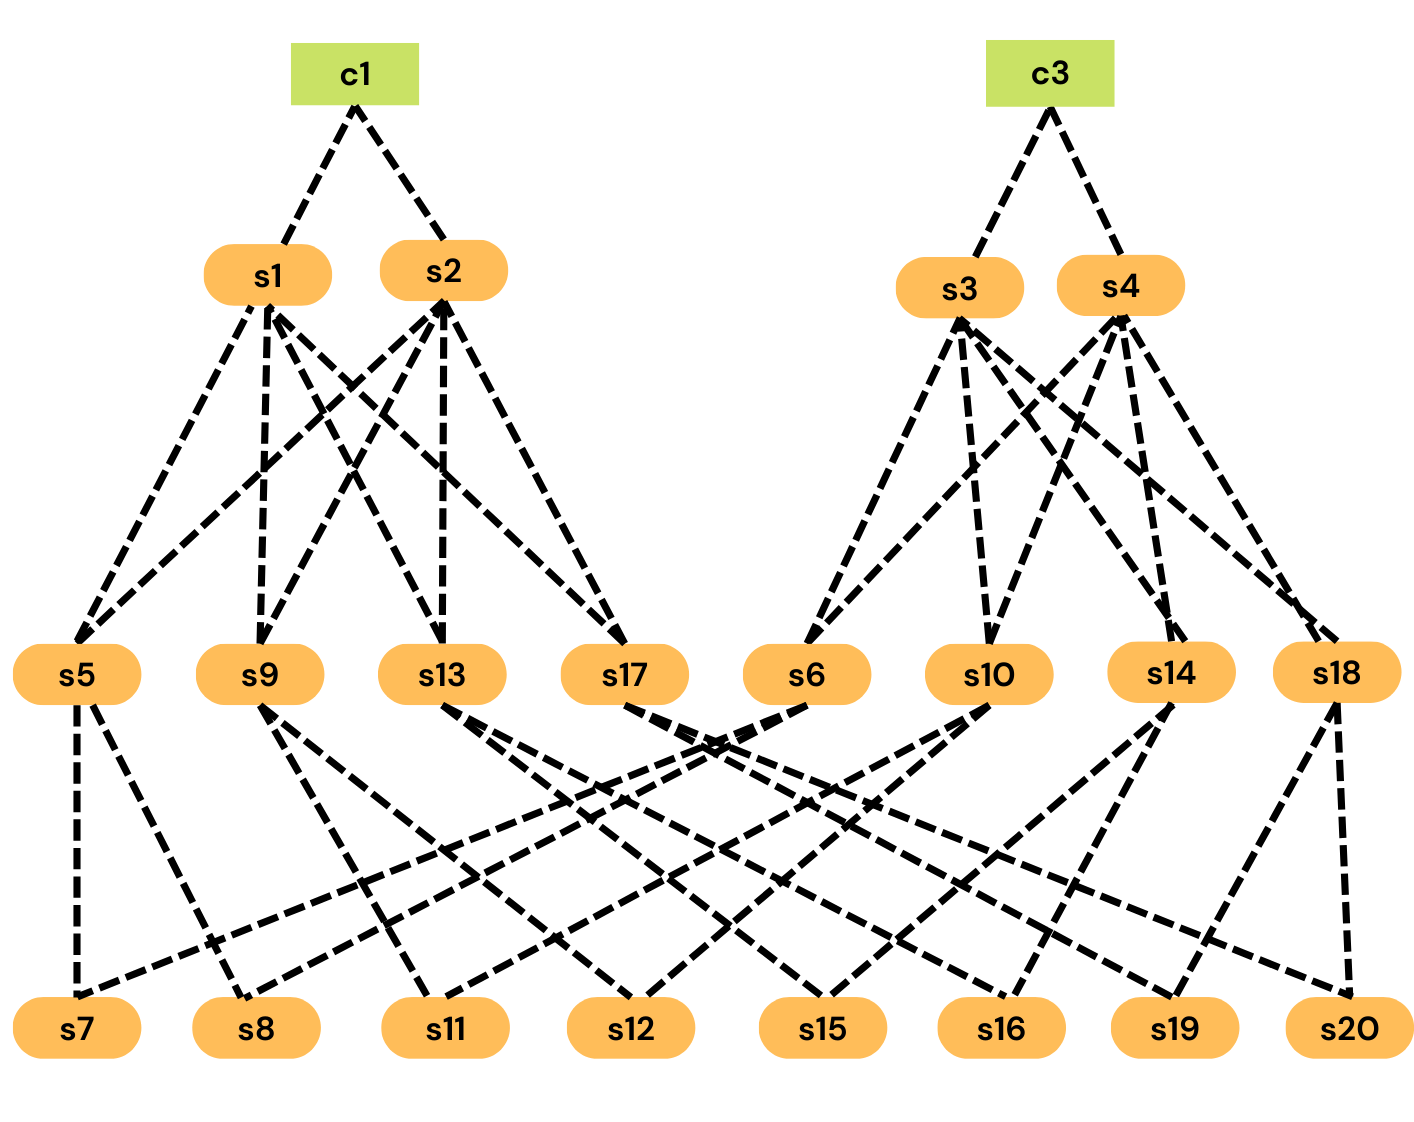
\includegraphics[width=13cm, keepaspectratio]{img/e4_2}
		\caption{Cuarto escenario con 2 controladores y 20 switches}
		\label{figura:e4_2}
	\end{figure}
	
	
	\begin{figure}[H]
		\centering
		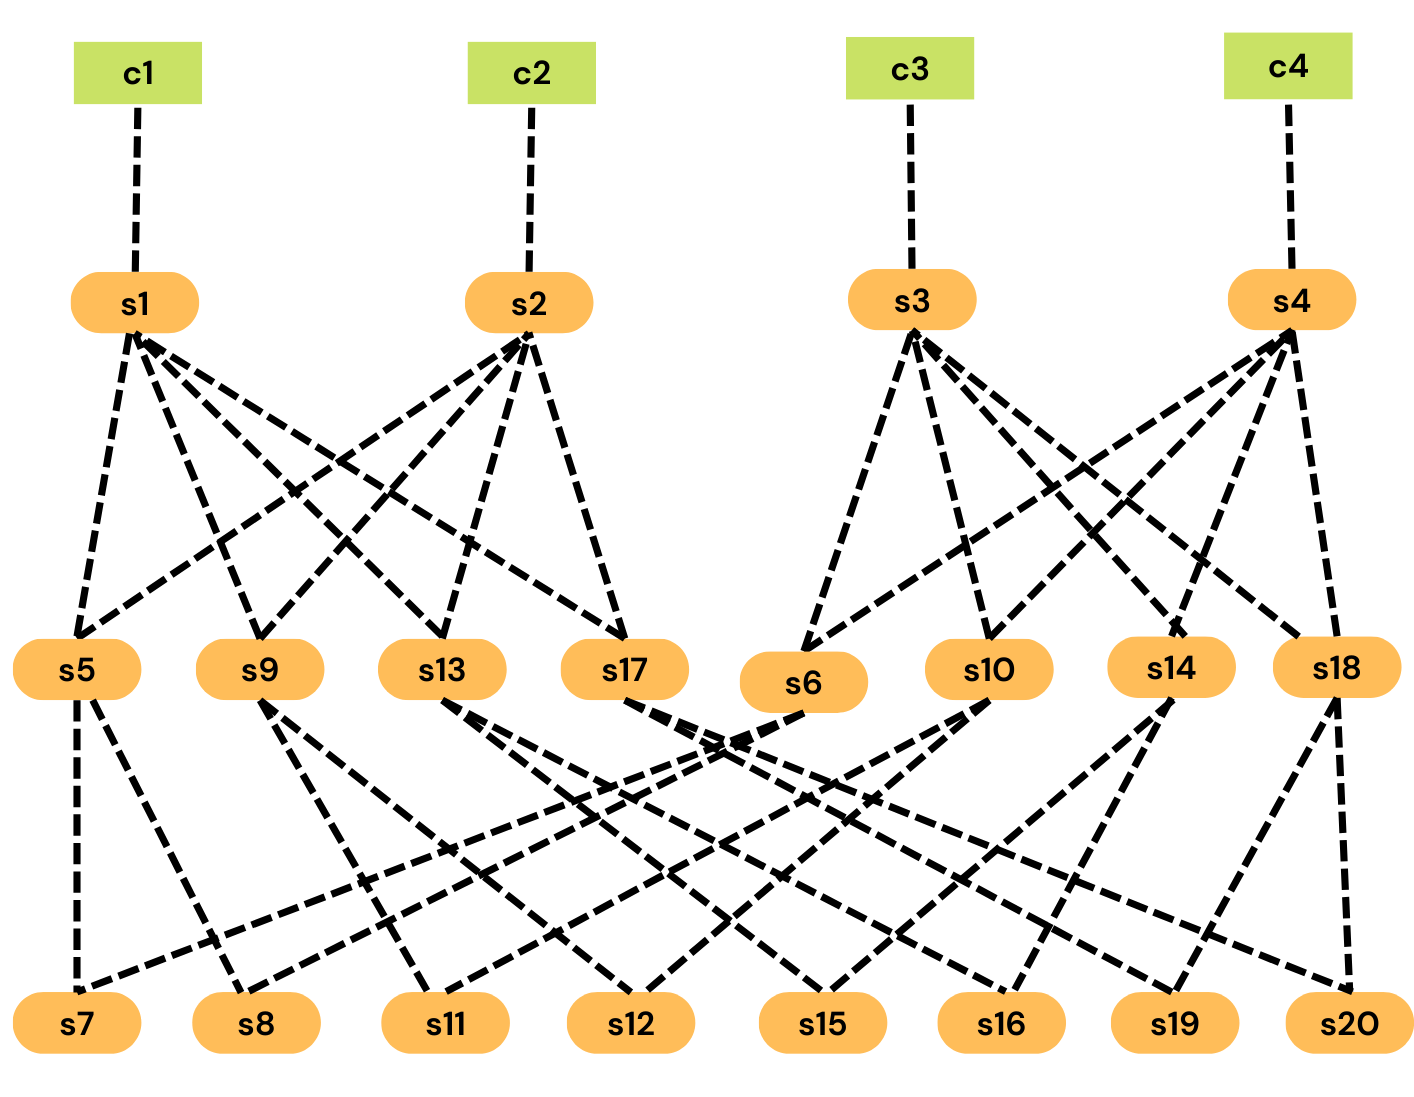
\includegraphics[width=13cm, keepaspectratio]{img/e4_3}
		\caption{Cuarto escenario con 4 controladores y 20 switches}
		\label{figura:e4_3}
	\end{figure}
	
En las figuras 5.22 y 5.23 podemos observar la comparación del escenario con 1 y 2 controladores en tiempos y medias. Con estos resultados vemos que no simplemente importa que se acorten los saltos, sino que también es importante la carga de trabajo que va a tener cada controlador, ya que el tiempo máximo de conexión en los switches se ha reducido en 0.168 segundos, siendo el sistema un 47.19 \% mas rápido con 2 controladores que con 1. Teniendo en cuenta que la carga de trabajo se ha repartido entre 2, podemos observar que para escenarios complejos, cuantos mas controladores haya, mucho más rápida será la configuración de los switches, independientemente de si se acortan los saltos o no.
		
		
	
	
	\begin{figure}[H]
		\centering
		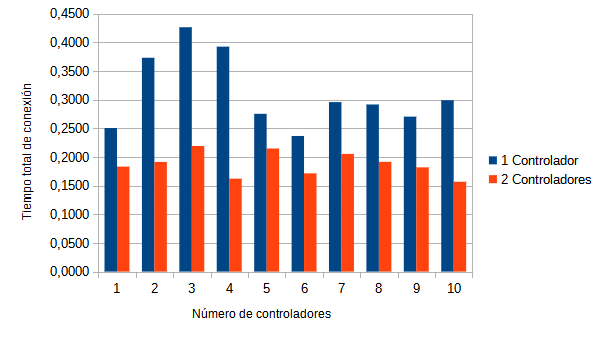
\includegraphics[width=13cm, keepaspectratio]{img/comparativaescenario4}
		\caption{Tiempo que tardan todos los switches del escenario 4 en estar gestionados por un controlador.}
		\label{figura:comparativaescenario4}
	\end{figure}
	
	\begin{figure}[H]
		\centering
		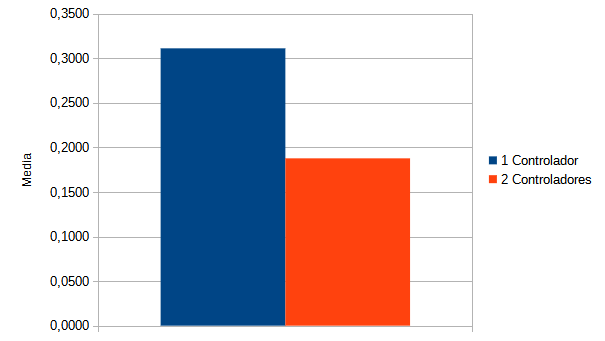
\includegraphics[width=13cm, keepaspectratio]{img/comparativamediaescenario4}
		\caption{Comparativa de media de tiempos en conseguir que todos los switches del escenario 4 estén gestionados por un controlador.}
		\label{figura:mediaescenario4}
	\end{figure}
	

	Y como vemos en las siguientes gráficas, también hay bastante diferencia en la mediana y la varianza. Ya que al haber 2 controladores y tanta conexión, es difícil que haya tiempos muy altos, de ahí que se reduzca la mediana y sobretodo la varianza.
	
%	Además, hemos comprobado que por lo general el reparto de switches entre los controladores se ha realizado de forma correcta.
\begin{figure}[H]
	\centering
	
	\subfigure[Comparativa de medianas en conseguir que todos los switches del escenario 4 estén gestionados por un controlador]{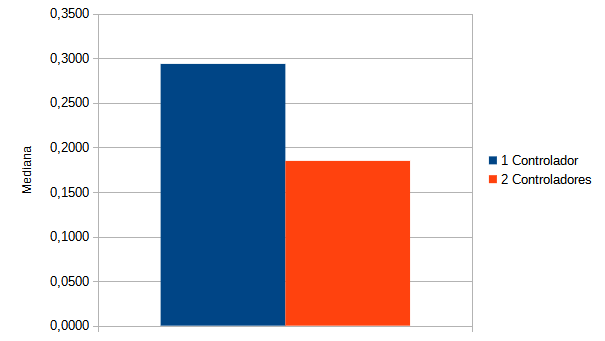
\includegraphics[width=0.45\textwidth]{img/comparativamedianaescenario4}}
	\hfill
	\subfigure[Comparativa de varianza en conseguir que todos los switches del escenario 4 estén gestionados por un controlador]{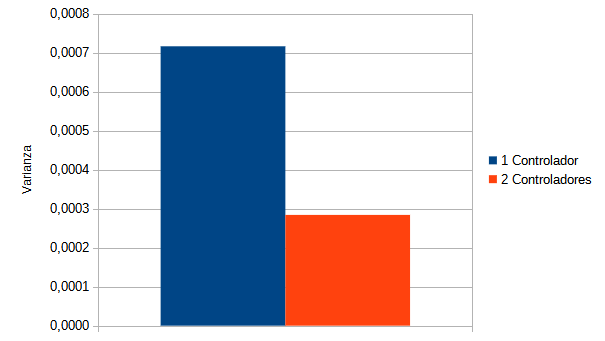
\includegraphics[width=0.45\textwidth]{img/comparativavarianzaescenario4}}
	\hfill
\end{figure}
	
		Además, viendo la figura 5.24 hemos comprobado que el reparto de switches entre los controladores se ha realizado de forma previsible y como se intuía al principio- El primer controlador acapara mas switches conectados en cada experimento, debido a que en este escenario mas complejo, el retraso que tiene el segundo controlador en arrancar da suficiente tiempo al primero para adelantarse en las conexiones.
		
	\begin{figure}[H]
		\centering
		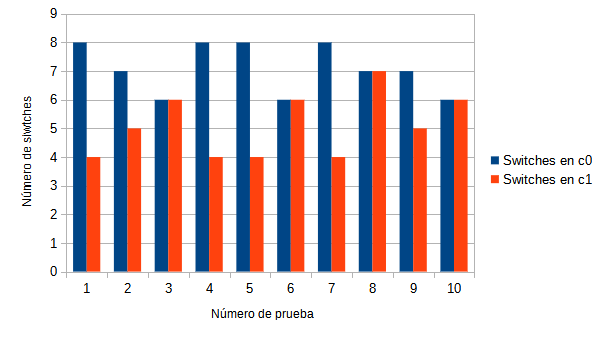
\includegraphics[width=16cm, keepaspectratio]{img/switchesporcontrollerescenario3}
		\caption{Número de switches por controlador.}
		\label{figura:switchesporcontrollerescenario4}
	\end{figure}
	

	
En la figura 5.25 podemos observar una comparativa del escenario con 1, 2 y 4 controladores.
	
	\begin{figure}[H]
		\centering
		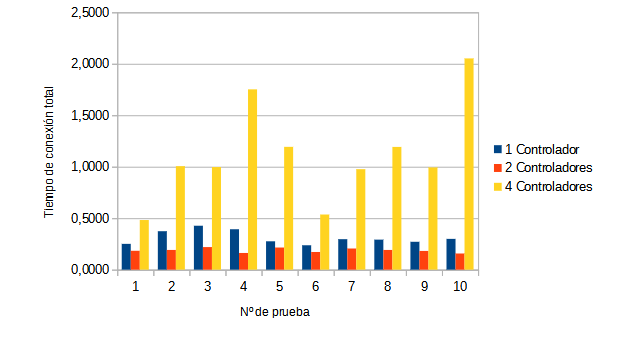
\includegraphics[width=16cm, keepaspectratio]{img/comparativaFail}
		\caption{Tiempo que tardan todos los switches del escenario 4 en estar gestionados por un controlador con 3 opciones diferentes.}
		\label{figura:comparativaFail}
	\end{figure}
	
	En este gráfico, esta vez vemos que no ha habido mejora, sino que ha habido un empeoramiento muy  significativo. Puede ser debido a problemas con la máquina donde se realizaban los experimentos, o debido al propio experimento. Lo que en ambos casos puede significar que una sobrecarga de controladores, puede perjudicar el funcionamiento de este escenario.
	
	
	%%%%%%%%%%%%%%%%%%%%%%%%%%%%%%%%%%%%%%%%%%%%%%%%%%%%%%%%%%%%%%%%%%%%%%%%%%%%%%%%
	%%%%%%%%%%%%%%%%%%%%%%%%%%%%%%%%%%%%%%%%%%%%%%%%%%%%%%%%%%%%%%%%%%%%%%%%%%%%%%%%
	% CONCLUSIONES %
	%%%%%%%%%%%%%%%%%%%%%%%%%%%%%%%%%%%%%%%%%%%%%%%%%%%%%%%%%%%%%%%%%%%%%%%%%%%%%%%%
	
	\clearpage
	\chapter{Conclusiones}
	\label{chap:conclusiones}
	
	Como conclusión de lo visto en los diferentes experimentos, podemos confirmar que añadir un controlador a un escenario va a ayudar, en la gran mayoría de los casos, a minimizar tiempos de conexión. Además, dicho tiempo mejorará cuanto mas lejos estén los nuevos controladores de los actuales del sistema, ya que los controladores tendrán que dar menos saltos para llegar a los switches que eran mas lejanos, y por tanto, se reducirá el tiempo final.  
	
	\section{Consecución de objetivos}
	\label{sec:consecucion-objetivos}
	
	Como pudimos ver en el apartado ~\ref{chap:objetivos}, se pretendía conocer mejor el funcionamiento de Periplus con respecto al número de controladores, y en cada escenario hemos podido ver nuevas casuísticas que nos han ido aportando nueva información sobre el ya mencionado protocolo de comunicación. Con el primer escenario, que era el más pequeño y el que se puede estudiar más en profundidad, ya se pudo vislumbrar cómo iban a funcionar el resto de escenarios, que en efecto, han confirmado las hipótesis que planteamos con dichos resultados del escenario 1. Y es que, añadir nuevos controladores, en los puntos mas alejados del o los controladores que tuviésemos, va a reducir considerablemente el tiempo de inicialización, ademas de un reparto mas equitativo de switches por controlador.
	
	Asimismo, con el ultimo experimento, hemos comprobado que no es siempre productivo añadir controladores, ya que una sobrecarga de éstos puede empeorar significativamente nuestros resultados debido a que pese a acortar los caminos, también aporta más complejidad y mas componentes, que es algo que en algunos escenarios puede perjudicar mas que beneficiar.
	
	\section{Aplicación de lo aprendido}
	\label{sec:aplicacion}
	A lo largo del presente Trabajo de Fin de Grado he podido aplicar conocimientos adquiridos en las siguientes asignaturas: 
	\begin{enumerate}
		\item Arquitectura de Redes de Ordenadores. Primer contacto con las redes de ordenadores, protocolos de comunicación, etc.
		\item Sistemas Telemáticos. Continuación de Arquitectura de Redes de Ordenadores, donde se profundizaba mas en materia.
	\end{enumerate}
	
	
	\section{Lecciones aprendidas}
	\label{sec:lecciones_aprendidas}
	
	A raíz de empezar a investigar para poder realizar el presente Trabajo de Fin de Grado hemos podido adquirir conocimientos en lo que respecta a:
	
	\begin{enumerate}
		\item OpenFlow. Al ser el elemento principal de esta investigación, la mayor parte de conocimiento que he adquirido ha sido sobre el protocolo de comunicación OpenFlow. El protocolo OpenFlow establece una comunicación entre el controlador y los dispositivos de red mediante mensajes definidos. El controlador puede enviar instrucciones a los dispositivos de red, como reglas de enrutamiento o de flujo, y recibir información sobre el estado de la red, como estadísticas de tráfico. Esto permite una gestión centralizada y programable de la red, lo que facilita la implementación de políticas de red, la optimización del tráfico y la resolución de problemas.
		\item LaTeX, ya que la memoria se ha realizado íntegramente con LaTeX. Con la ayuda de la plantilla hecha por el profesor Gregorio Robles y sus indicaciones, ha sido bastante sencillo realizar la documentación con dicha herramienta.
		\item Python. Pese a que el trabajo en si no tenía programación, he tenido que aprender las bases del lenguaje para entender los Scripts que se han utilizado tanto para definir los escenarios como para la realización de las pruebas.
		\item Desarrollar actitudes de investigación.
		
	\end{enumerate}
	
	
	\section{Trabajos futuros}
	\label{sec:trabajos_futuros}
	
	Tras realizar el presente TFG y visto lo aprendido y analizado el contenido del mismo, considero que sería una buena opción a tener en cuenta el optimizar los escenarios del sistema, creando lógica en los controladores, con el objetivo de evitar saturar determinados switches. Asimismo opino que podría ser interesante investigar sobre hasta que punto es factible añadir controladores extra a un escenario, ya que posiblemente llegue un punto que la mejora no sea lo suficientemente satisfactoria. 
	Además, debido a lo ocurrido en el último experimento, creo que sería muy interesante estudiar escenarios complejos con diferente número de controladores, y ver como afectan estos controladores extras a la estabilidad del escenario y los tiempos de resolución de incidencias, ya que quizás se pueda sacar algún tipo de relación o ecuación para calcular el número óptimo de controladores por switches o por distancia.
	
	
	%%%%%%%%%%%%%%%%%%%%%%%%%%%%%%%%%%%%%%%%%%%%%%%%%%%%%%%%%%%%%%%%%%%%%%%%%%%%%%%%
	%%%%%%%%%%%%%%%%%%%%%%%%%%%%%%%%%%%%%%%%%%%%%%%%%%%%%%%%%%%%%%%%%%%%%%%%%%%%%%%%
	% APÉNDICE(S) %
	%%%%%%%%%%%%%%%%%%%%%%%%%%%%%%%%%%%%%%%%%%%%%%%%%%%%%%%%%%%%%%%%%%%%%%%%%%%%%%%%
	
	\cleardoublepage
	
	%%%%%%%%%%%%%%%%%%%%%%%%%%%%%%%%%%%%%%%%%%%%%%%%%%%%%%%%%%%%%%%%%%%%%%%%%%%%%%%%
	%%%%%%%%%%%%%%%%%%%%%%%%%%%%%%%%%%%%%%%%%%%%%%%%%%%%%%%%%%%%%%%%%%%%%%%%%%%%%%%%
	% BIBLIOGRAFIA %
	%%%%%%%%%%%%%%%%%%%%%%%%%%%%%%%%%%%%%%%%%%%%%%%%%%%%%%%%%%%%%%%%%%%%%%%%%%%%%%%%
	
	\cleardoublepage
	
	% Las siguientes dos instrucciones es todo lo que necesitas
	% para incluir las citas en la memoria
	\bibliographystyle{abbrv}
	\bibliography{memoria} 
	
	[1]  A robust and reactive
	OpenFlow In-Band SDN Control Plane
	Version 0.1. Autores Pedro de las Heras y Eva María Castro. 2022
	
	[2]  Página informativa de OpenFlow https://noviflow.com/the-basics-of-sdn-and-the-openflow-network-architecture/ 
		
	[3]  Guía de LaTex.  https://github.com/gregoriorobles/plantilla-memoria/blob/master/memoria.tex
	
	[4]  Foundations of Modern Networking: SDN, NFV, QoE, IoT, and Cloud By William Stallings 2015
	
	[5]  Introducción a namespaces https://man7.org/linux/man-pages/man8/ip-netns.8.html
	
	[6]  Introducción a openvswitch http://openvswitch.org
	
	[7]  Introducción a Mininet http://mininet.org
	
	[8]  Continuación Mininet https://www.youtube.com/live/90fBCO1MMTA?si=uVvZdvl4D7t8ntFw
	
	[9]  Documentación de Networking http://docs.openstack.org
	
	[10] Documentación Linux Networking https://www.opencloudblog.com/
	
	[11] Documentación Faucet https://docs.faucet.nz/en/latest/tutorials/
 	
	 % memoria.bib es el nombre del fichero que contiene
	% las referencias bibliográficas. Abre ese fichero y mira el formato que tiene,
	% que se conoce como BibTeX. Hay muchos sitios que exportan referencias en
	% formato BibTeX. Prueba a buscar en http://scholar.google.com por referencias
	% y verás que lo puedes hacer de manera sencilla.
	% Más información: 
	% http://texblog.org/2014/04/22/using-google-scholar-to-download-bibtex-citations/
	
\end{document}
